\documentclass{classrep}
\usepackage[utf8]{inputenc}
\frenchspacing

\usepackage{graphicx}
\usepackage[usenames,dvipsnames]{color}
\usepackage[hidelinks]{hyperref}
\usepackage{lmodern}
\usepackage{graphicx}
\usepackage{placeins}
\usepackage{url}
\usepackage{amsmath, amssymb, mathtools}
\usepackage{listings}
\usepackage{fancyhdr, lastpage}

\pagestyle{fancyplain}
\fancyhf{}
\renewcommand{\headrulewidth}{0pt}
\cfoot{\thepage\ / \pageref*{LastPage}}

%--------------------------------------------------------------------------------------%
\studycycle{Informatyka stosowana, studia dzienne, II st.}
\coursesemester{II}

\coursename{Przetwarzanie i analiza dużych zbiorów danych}
\courseyear{2021/2022}

\courseteacher{mgr inż. Rafał Woźniak}
\coursegroup{Czwartek, 15:45}

\author{%
    \studentinfo[239661@edu.p.lodz.pl]{Szymon Gruda}{239661}\\
    \studentinfo[239671@edu.p.lodz.pl]{Jan Karwowski}{239671}\\
    \studentinfo[239673@edu.p.lodz.pl]{Michał Kidawa}{239673}\\
    \studentinfo[239676@edu.p.lodz.pl]{Kamil Kowalewski}{239676}\\
}

\title{Checkpoint 4}

\begin{document}
    \maketitle
    \thispagestyle{fancyplain}

    \tableofcontents
    \newpage

    \section{Wprowadzenie} {
        Głównym celem projektu jest przeprowadzenie kompleksowej analizy zbioru
        \textit{NYPD Complaint Data Historic} \cite{nypd_dataset} poprzez wstępną
        analizę zbioru danych, zaobserwowanie zależności pomiędzy danymi i określenie
        celów projektu, których realizacja da odpowiedź na podstawione cele badawcze i
        na jej podstawie zostaną wyciągnie wnioski.
    }

    \section{Podział obowiązków w zespole} {
        \begin{itemize}
            \item Szymon Gruda - Realizacja celu "Klasyfikacja rodzaju lub poziomu przestępstwa"
            \item Jan Karwowski - Realizacja celu "Regresja godziny wystąpienia zdarzenia"
            \item Michał Kidawa - Realizacja celu "Grupowanie przestępstw na podstawie podzbiorów cech"
            \item Kamil Kowalewski - Przygotowywanie preprocessingu, miejsca oraz infrastruktury do realizacji celów badawczych. Pomoc programistyczna oraz techniczna dla pozostałych członków zespołu w badaniach
        \end{itemize}
    }

    \section{Charakterystyka zbioru danych} {

        \subsection{Przegląd pierwotnie dostępnych kolumn} {
            Zbiór danych zawiera ponad 7 mln. (7375993) wierszy i 35 kolumn różnego typu, głównie dane kategorialne. Poniżej wypisane zostały wszystkie dostępne kolumny, pogrupowane tematycznie, wraz z informacją kolejno o liczbie unikalnych wartości (włącznie z NaN) i brakujących wartości (NaN) w danej kolumnie.
        % @formatter:off
            \begin{enumerate}
                \item Identyfikator
                \begin{itemize}
                    \item CMPLNT\_NUM (unikalnych 7373143, brakujących 0) - Losowo generowany trwały identyfikator dla każdego zgłoszenia
                \end{itemize}
                \item Data i czas zdarzenia
                \begin{itemize}
                    \item CMPLNT\_FR\_DT (unikalnych 8607, brakujących 655) - Dokładna data wystąpienia zgłoszonego zdarzenia (lub data początkowa wystąpienia, jeżeli CMPLNT\_TO\_DT istnieje)
                    \item CMPLNT\_FR\_TM (unikalnych 1442, brakujących 48) - Dokładny czas wystąpienia zgłoszonego zdarzenia (lub czas rozpoczęcia wystąpienia, jeżeli CMPLNT\_TO\_TM istnieje)
                    \item CMPLNT\_TO\_DT (unikalnych 6826, brakujących 1704204) - Data końcowa wystąpienia zgłoszonego zdarzenia, jeżeli dokładny czas wystąpienia nie jest znany
                    \item CMPLNT\_TO\_TM (unikalnych 1442, brakujących 1699541) - Końcowy czas wystąpienia zgłoszonego zdarzenia, jeżeli dokładny czas wystąpienia nie jest znany
                \end{itemize}
                \item Data i czas zgłoszenia
                \begin{itemize}
                    \item RPT\_DT (unikalnych 5479, brakujących 0) - Data zgłoszenia zdarzenia na policję
                \end{itemize}
                \item Typ i opis wykroczenia/przestępstwa
                \begin{itemize}
                    \item KY\_CD (unikalnych 74, brakujących 0) - Trzycyfrowy kod klasyfikacji wykroczeń
                    \item OFNS\_DESC (unikalnych 72, brakujących 18823) - Opis wykroczenia odpowiadający kodowi klucza
                    \item PD\_CD (unikalnych 433, brakujących 6278) - Trzycyfrowy kod klasyfikacji wewnętrznej (bardziej szczegółowy niż Key Code)
                    \item PD\_DESC (unikalnych 423, brakujących 6278) - Opis wewnętrznej klasyfikacji odpowiadającej kodowi PD (bardziej szczegółowy niż opis przestępstwa)
                    \item LAW\_CAT\_CD (unikalnych 3, brakujących 0) - Poziom wykroczenia: przestępstwo, wykroczenie, naruszenie
                \end{itemize}
                \item Czy się udało
                \begin{itemize}
                    \item CRM\_ATPT\_CPTD\_CD (unikalnych 3, brakujących 7) - Status, czy przestępstwo zostało dokonane czy była próba jego popełnienia lub czy zostało ono przerwane
                \end{itemize}
                \item Otoczenie zdarzenia
                \begin{itemize}
                    \item PREM\_TYP\_DESC (unikalnych 75, brakujących 40745) - Rodzaj otoczenia; sklep spożywczy, domek jednorodzinny, ulica itp.
                    \item LOC\_OF\_OCCUR\_DESC (unikalnych 6, brakujących 1543800) - Lokalizacja w stosunku do otoczenia; wewnątrz, naprzeciw, z przodu, z tyłu
                \end{itemize}
                \item Lokalizacja zdarzenia
                \begin{itemize}
                    \item ADDR\_PCT\_CD (unikalnych 78, brakujących 2166) - Posterunek
                    \item BORO\_NM (unikalnych 6, brakujących 11329) - Dzielnica
                    \item JURIS\_DESC (unikalnych 25, brakujących 0) - Opis kodu jurysdykcji
                    \item JURISDICTION\_CODE (unikalnych 26, brakujących 6278) - Kod jurysdykcji na której miało miejsce to zdarzenie
                    \item PARKS\_NM (unikalnych 1206, brakujących 7348330) - Nazwa parku, placu zabaw lub terenów zielonych w Nowym Jorku, jeśli dotyczy (parki stanowe nie są uwzględnione)
                    \item HADEVELOPT (unikalnych 280, brakujących 7029181) - Nazwa osiedla NYCHA miejsca zdarzenia, jeśli dotyczy
                    \item HOUSING\_PSA (unikalnych 5088, brakujących 6809283) - Kod poziomu rozwoju
                    \item X\_COORD\_CD (unikalnych 71344, brakujących 17339) - Współrzędna X dla układu współrzędnych płaszczyzny stanu Nowy Jork, strefa Long Island, NAD 83, jednostki w stopach (FIPS 3104)
                    \item Y\_COORD\_CD (unikalnych 73934, brakujących 17339) - Współrzędna Y dla układu współrzędnych płaszczyzny stanu Nowy Jork, strefa Long Island, NAD 83, jednostki w stopach (FIPS 3104)
                    \item TRANSIT\_DISTRICT (unikalnych 13, brakujących 7212494) - Okręg tranzytowy, w którym doszło do wykroczenia.
                    \item Latitude (unikalnych 205540, brakujących 17339) - Współrzędna szerokości geograficznej środkowego bloku dla globalnego układu współrzędnych, WGS 1984, stopnie dziesiętne (EPSG 4326)
                    \item Longitude (unikalnych 201312, brakujących 17339) - Współrzędna długości bloku środkowego dla globalnego układu współrzędnych, WGS 1984, stopnie dziesiętne (EPSG 4326)
                    \item Lat\_Lon (unikalnych 198553, brakujących 17339) - Punkt lokalizacji geoprzestrzennej (łącznie szerokość i długość geograficzna)
                    \item PATROL\_BORO (unikalnych 9, brakujących 6735) - Nazwa dzielnicy patrolowej, w której doszło do incydentu
                    \item STATION\_NAME (unikalnych 373, brakujących 7212494) - Nazwa stacji tranzytowej
                \end{itemize}
                \item Cechy podejrzanego
                \begin{itemize}
                    \item SUSP\_AGE\_GROUP (unikalnych 112, brakujących 4795235) - Grupa wiekowa podejrzanego
                    \item SUSP\_RACE (unikalnych 9, brakujących 3426694) - Rasa podejrzanego
                    \item SUSP\_SEX (unikalnych 4, brakujących 3560008) - Płeć podejrzanego
                \end{itemize}
                \item Cechy ofiary
                \begin{itemize}
                    \item VIC\_AGE\_GROUP (unikalnych 203, brakujących 1638445) - Grupa wiekowa ofiary
                    \item VIC\_RACE (unikalnych 9, brakujących 309) - Rasa ofiary
                    \item VIC\_SEX (unikalnych 6, brakujących 308) - Płeć ofiary
                \end{itemize}
            \end{enumerate}
        % @formatter:on
        }

        \subsection{Szczegółowa charakterystyka wybranych kolumn} {
            
            Poniżej przedstawiona została bardziej szczegółowa charakterystyka wybranych kolumn ze zbioru danych, zwłaszcza rozkłady dostępnych w nich wartości (histogramy). Omówione również zostały możliwości wstępnego oczyszczenia i przetwarzania danych, przed właściwą analizą (szczegółowy preprocessing jest omówiony osobno dla każdego celu). Wspomniane zostały także kolumny, które wydają się być nieprzydatne i nie zostały wykorzystane w dalszej analizie.

            \subsubsection{Data oraz czas zdarzenia i zgłoszenia} {
                
                Jako, że data i czas zdarzenia co do swojej oryginalnej wartości nie niosą praktycznie żadnej przydatnej informacji, niezbędne jest dla tych kolumn przeprowadzenie prostej ekstrakcji cech. Podstawowymi cechami, które można wyekstrahować z daty i czasu wystąpienia zdarzenia jest pora dnia, dzień tygodnia czy pora roku. Dla rekordów, dla których znany jest czas zakończenia zdarzenia, można wyekstrahować również czas trwania zdarzenia.
                
                \begin{figure}[!htbp]
                    \centering
                    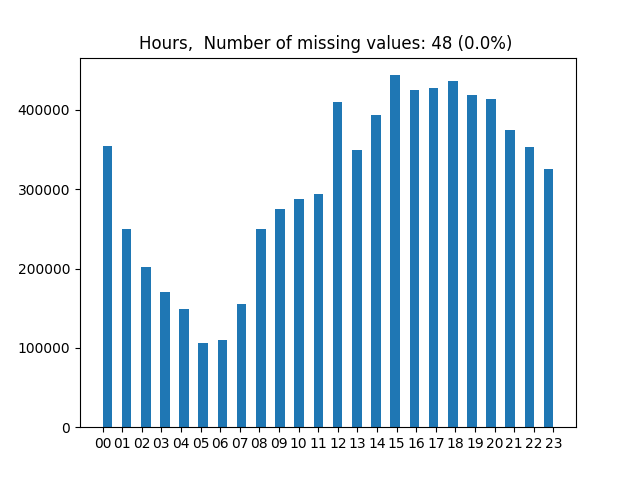
\includegraphics[width=0.9\textwidth]{img/Hours-133549.png}
                    \caption{Histogram liczby zdarzeń w zależności od godziny}
                    \label{hist_hours}
                \end{figure}
                \begin{figure}[!htbp]
                    \centering
                    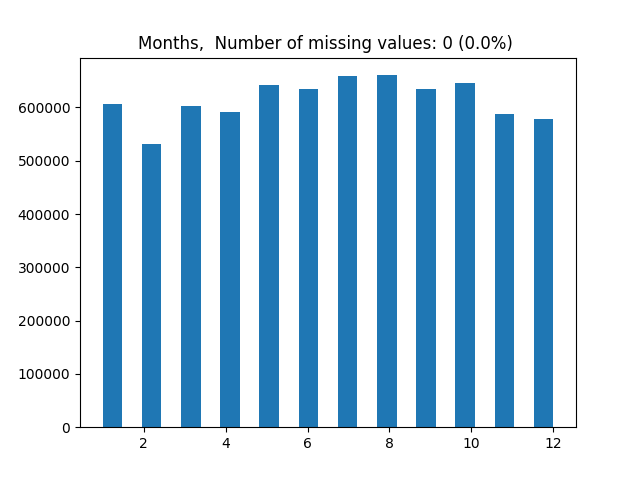
\includegraphics[width=0.9\textwidth]{img/Months-133554.png}
                    \caption{Histogram liczby zdarzeń w zależności od miesiąca (pory roku)}
                    \label{hist_months}
                \end{figure}
                \FloatBarrier

                Na podstawie rysunku \ref{hist_hours} można zaobserwować, że największa
                liczba przestępstw/wykroczeń miała miejsce w godzinach popołudniowych,
                natomiast najmniejsza w godzinach wczesnoporonnych tzn godzina 5 i 6 rano. Na podstawie rysunku \ref{hist_months} można zaobserwować, że wyniki
                liczby przestępstw/wykroczeń są do siebie zbliżone natomiast większa
                liczba była w czasie miesięcy letnich.
                
                Parametry rozkładu czasu trwania zdarzenia to:
                \begin{itemize}
                    \item średnia = 248h
                    \item odchylenie standardowe = 4769h (prawie 200 dni)
                    \item minimum = -122h (błąd - należy dodatkowo oczyścić dane)
                    \item maksimum = ponad 10 lat
                    \item mediana = 1380s
                    \item centyl 80 = 11h
                    \item centyl 90 = 40h
                \end{itemize}
                Jak widać rozkład ten jest bardzo nierównomierny i zwłaszcza próba estymacji tej wartości może okazać się trudna. Data zgłoszenia zdarzenia na policję nie niesie szczególnie istotnej wartości i nie jest wykorzystywana w dalszej analizie.
            }

            \subsubsection{Typ i opis zdarzenia} {
                Na podstawie rysunku \ref{hist_law_breaking_level} można zaobserwować,
                że największy odsetek stanowiły wykroczenia, na drugim miejscu
                uplasowały się przestępstwa natomiast najmniej było występków(jest to
                pośredni czyli między wykroczeniem a przestępstwem). Rysunki \ref{hist_ky_cd} oraz \ref{hist_pd_cd} pokazują, że zdecydowana większość zdarzeń mieści się w zaledwie kilku pierwszych (z kilkudziesięciu) kodów klasyfikacji zdarzenia.
                
                Kolumny zawierające słowne opisy przestępstwa odpowiadają praktycznie zawsze danem kodowi, tak więc na potrzeby działania algorytmu są zupełnie redundantne i nie będą wykorzystywane.
                
                Należy wspomnieć, że występuje bardzo silne powiązanie (reguła asocjacyjna) między kolejno PD\_CD -> KY\_CD oraz KY\_CD -> LAW\_CAT\_CD. Nie mają one 100\% pokrycia tak więc istnieją takie przestępstwa (KY\_CD), które występują we wszystkich trzech rodzajach. Jednakże pokrycie wspomnianych zależności jest bardzo duże i nie ma sensu przeprowadzać klasyfikacji LAW\_CAT\_CD w oparciu o KY\_CD.
                
                Wspomniane kolumny mają charakter kategorialny dlatego podczas ich wykorzystanie niezbędne będzie zastosowanie techniki \emph{one hot encoding}. Prawdopodobnie nie ma również sensu wykorzystywać wszystkich trzech informacji, zwłaszcza, że jak opisano wyżej, są one zależne jedna od drugiej.
                
                \begin{figure}[!htbp]
                    \centering
                    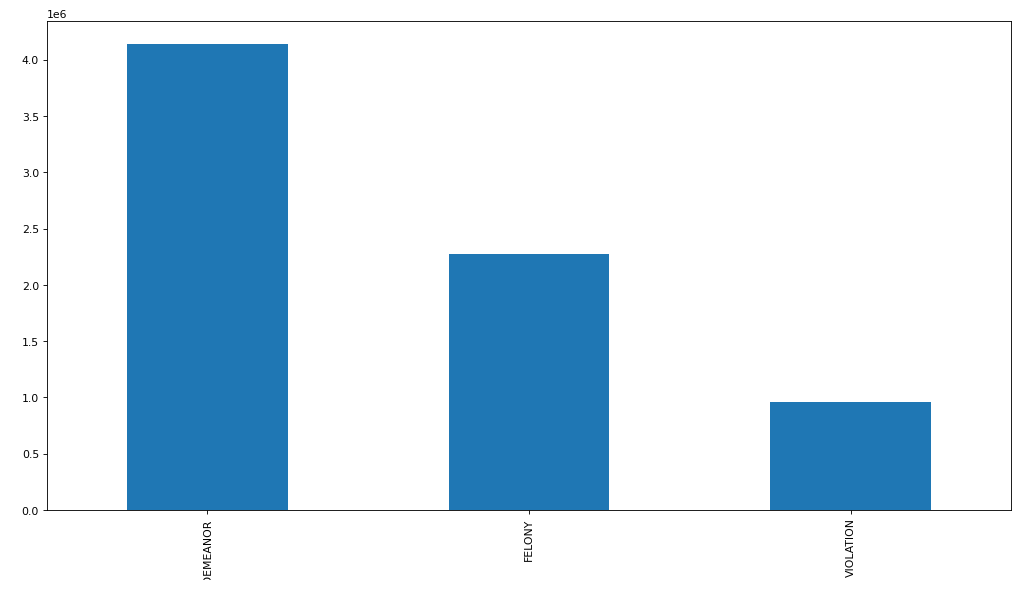
\includegraphics[width=0.9\textwidth]{img/hist_law_cat_cd.png}
                    \caption{Histogram liczby zdarzeń zależnie od jego typu}
                    \label{hist_law_breaking_level}
                \end{figure}
                \begin{figure}[!htbp]
                    \centering
                    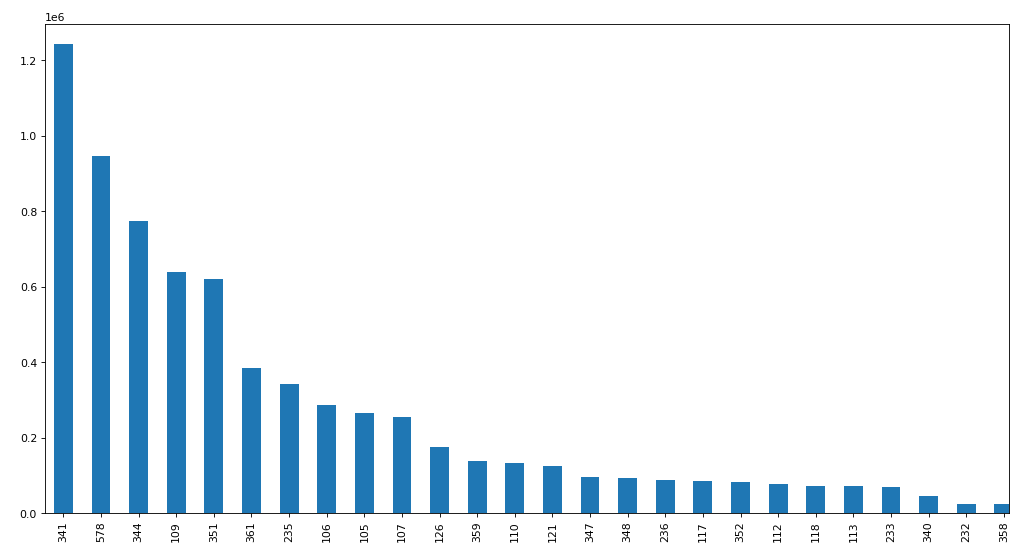
\includegraphics[width=\textwidth]{img/hist_ky_cd.png}
                    \caption{Początek histogramu liczby zdarzeń dla kodu zdarzenia (KY\_CD)}
                    \label{hist_ky_cd}
                \end{figure}
                \begin{figure}[!htbp]
                    \centering
                    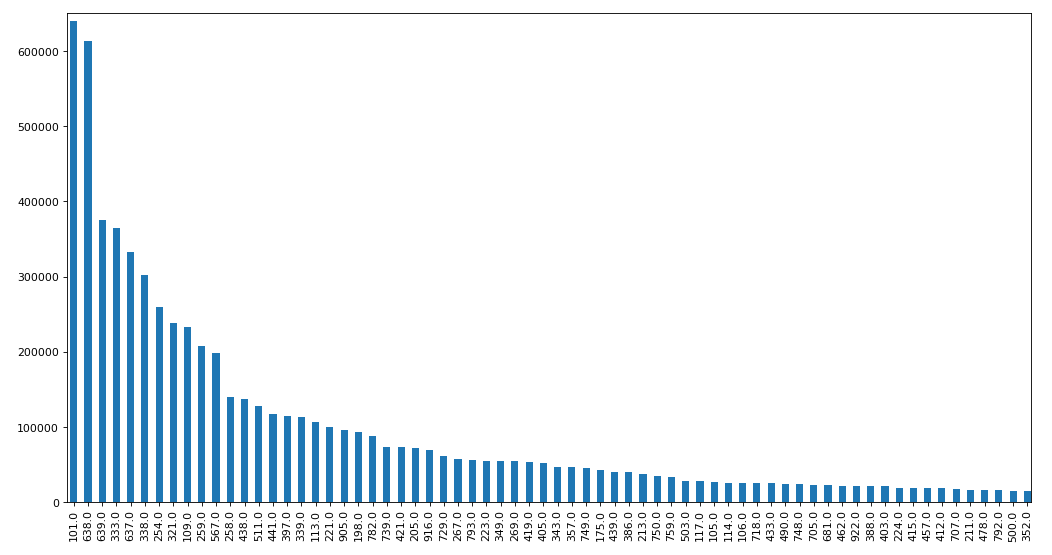
\includegraphics[width=\textwidth]{img/hist_pd_cd.png}
                    \caption{Początek histogramu liczby zdarzeń dla wewnętrznego kodu zdarzenia (PD\_CD)}
                    \label{hist_pd_cd}
                \end{figure}
                \FloatBarrier
            }

            \subsubsection{Czy się udało} {
                \begin{figure}[!htbp]
                    \centering
                    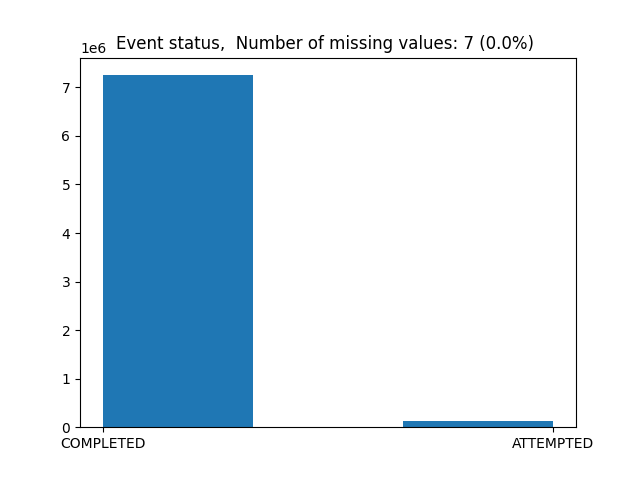
\includegraphics[width=0.85\textwidth]{img/Eventstatus-133630.png}
                    \caption{Histogram liczby zdarzeń w zależności od tego czy doszło ono do skutku czy zostało zatrzymane}
                    \label{hist_is_completed}
                \end{figure}
                \FloatBarrier
                Na podstawie rysunku \ref{hist_is_completed} można zaobserwować, że
                praktycznie wszystkie przestępstwa/wykroczenia zostały dokonane a
                naprawdę niewielki odsetek został udaremniony. Rozkład wartości w tej kolumnie jest więc silnie niezbalansowany.
                
                Wartość ta może zostać zakodowana w postaci pojedynczej kolumny z wartościami binarnymi.
            }

            \subsubsection{Otoczenie zdarzenia} {
                \begin{figure}[!htbp]
                    \centering
                    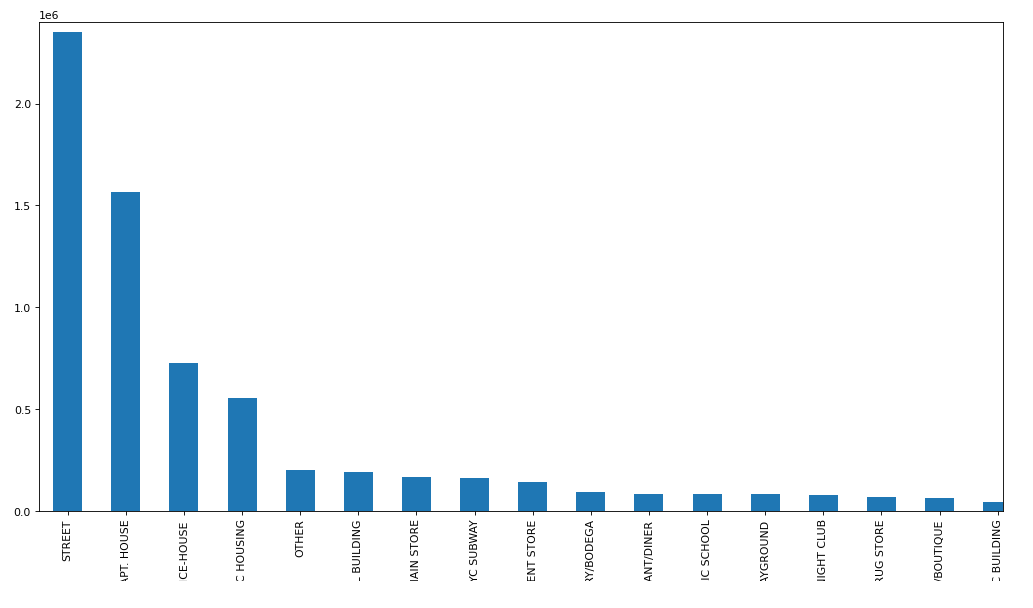
\includegraphics[width=\textwidth]{img/hist_prem.png}
                    \caption{Początek histogramu liczby zdarzeń dla otoczenia zdarzenia}
                    \label{hist_prem}
                \end{figure}
                \begin{figure}[!htbp]
                    \centering
                    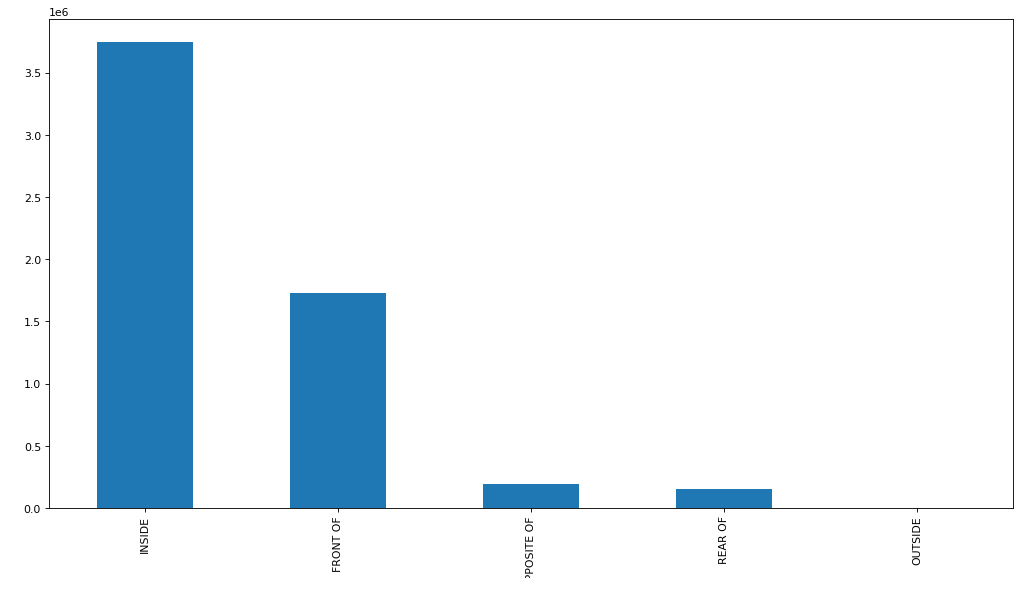
\includegraphics[width=\textwidth]{img/hist_loc_prem.png}
                    \caption{Histogram liczby zdarzeń dla lokalizacji w stosunku do otoczenia}
                    \label{hist_loc_prem}
                \end{figure}
                \FloatBarrier
                
                Na rysunku \ref{hist_prem} widać, że zdecydowana większość zdarzeń ma miejsce na ulicy i w domach. Z kolei rysunek \ref{hist_loc_prem} pokazuje, że najwięcej zdarzeń dzieje się wewnątrz jakiegoś miejsca. Jak widać rozkłady tych wartości znowu są silnie niezbalansowane. Typ danych pozostaje kategorialny i wymaga stosowania \emph{one hot encodingu}.
            }

            \subsubsection{Lokalizacja zdarzenia} {
                Informacje o dokładnej lokalizacji zdarzenia, w przeciwieństwie do wszystkich pozostałych informacji na temat zdarzenia dostępnych w tym zbiorze, nie mają charakteru uniwersalnego. Wykorzystanie ich oznaczałoby uzależnienie się od kontekstu miasta Noweg Jorku, z którego dane pochodzą. Dodatkowo dane te są redundantne, i w większości nie niosą żadnych przydatnych informacji dotyczących czy to rodzaju, czy też chwili popełnionego przestępstwa. Żadna z kolumn z tej grupy nie została wykorzystana w dalszej analizie.
            }

            \subsubsection{Cechy podejrzanego} {
                \begin{figure}[!htbp]
                    \centering
                    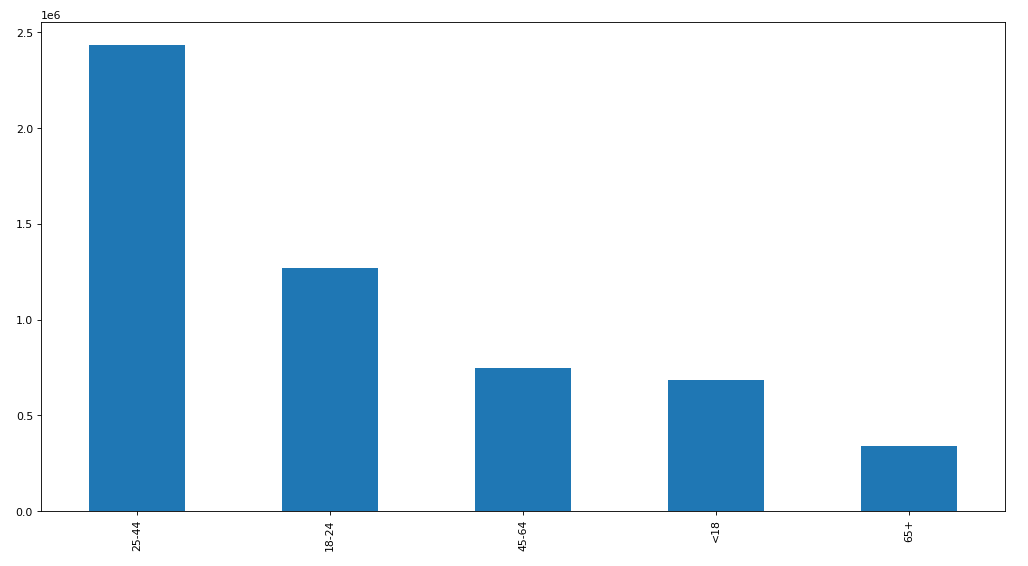
\includegraphics[width=0.85\textwidth]{img/hist_susp_age_group.png}
                    \caption{Histogram liczby zdarzeń popełnianych przez określoną grupę wiekową (po wstępnym oczyszczeniu zbioru).}
                    \label{hist_susp_age_group}
                \end{figure}
                \begin{figure}[!htbp]
                    \centering
                    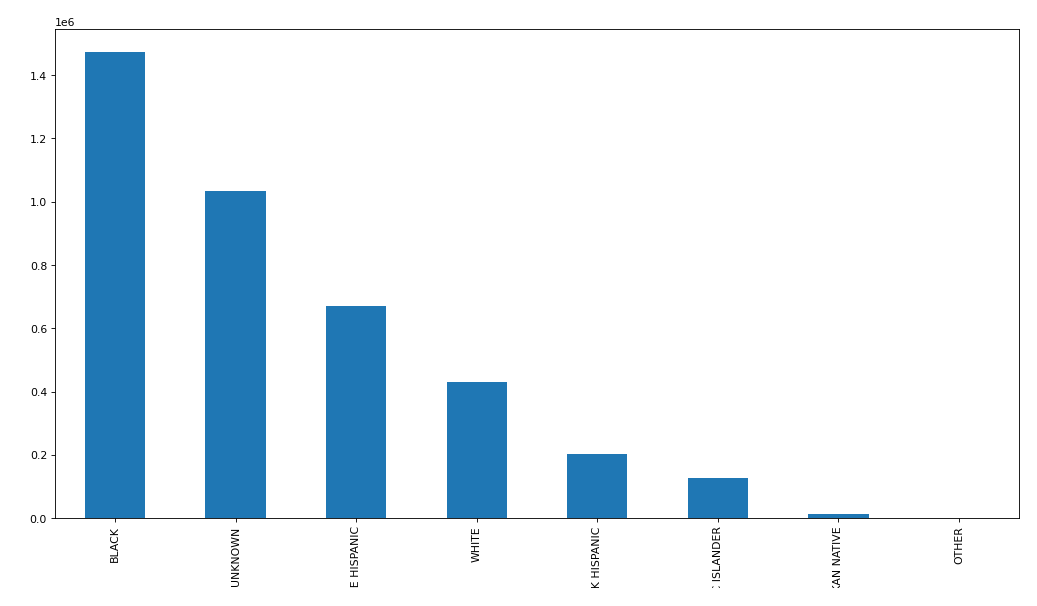
\includegraphics[width=0.85\textwidth]{img/hist_susp_race.png}
                    \caption{Histogram liczby zdarzeń popełnianych przez określoną rasę.}
                    \label{hist_susp_race}
                \end{figure}
                \begin{figure}[!htbp]
                    \centering
                    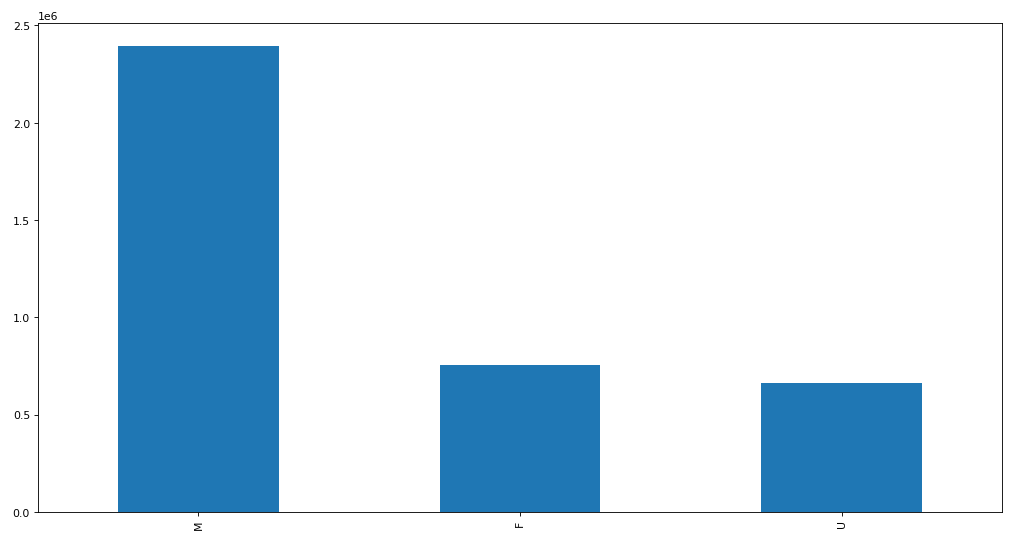
\includegraphics[width=0.85\textwidth]{img/hist_susp_sex.png}
                    \caption{Histogram liczby zdarzeń popełnianych przez określoną płeć.}
                    \label{hist_susp_sex}
                \end{figure}
                \FloatBarrier
                Na cechy podejrzanego składają się trzy wartości: grupa wiekowa, rasa oraz płeć. Grupa wiekowa jest silnie zanieczyszczona różnymi losowymi wartościami liczbowymi. Najprostszą metodą, stosowaną w większości przypadków, będzie ograniczenie liczby wartości do tych poprawnych (<18, 18-24, 25-44, 45-64, 65+) oraz wartości nieznanej (NaN). Rysunek \ref{hist_susp_age_group} przedstawia rozkład wieku podejrzanych po takim oczyszczeniu tych danych. Wynika z niego, że większość ludzi uwikłanych w różnego rodzaju przestępstwa i występki mają między 20 a 40 lat. Jest to również najliczniejsza grupa w społeczeństwie, stąd też przede wszystkim wynika ten rozkład (rozkład normalny). Kolejnym spostrzeżeniem, tym razem z rysunków \ref{hist_susp_race} i \ref{hist_susp_sex} jest fakt, że większość podejrzanych stanowią czarni mężczyźni.
            }

            \subsubsection{Cechy ofiary} {
                \begin{figure}[!htbp]
                    \centering
                    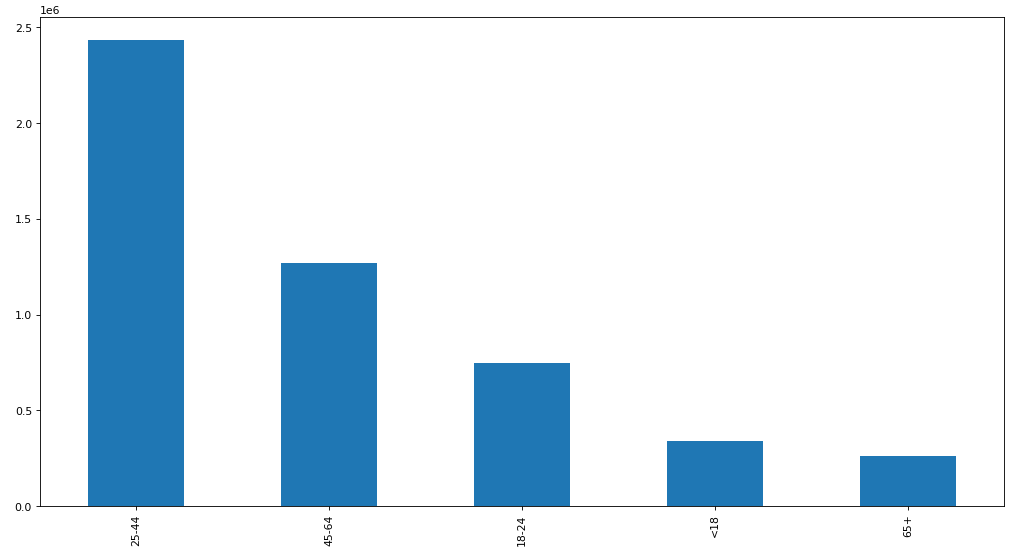
\includegraphics[width=0.85\textwidth]{img/hist_vic_age_group.png}
                    \caption{Histogram liczby zdarzeń dla danych grup wiekowych poszkodowanych (po wstępnym oczyszczeniu zbioru).}
                    \label{hist_vic_age_group}
                \end{figure}
                \begin{figure}[!htbp]
                    \centering
                    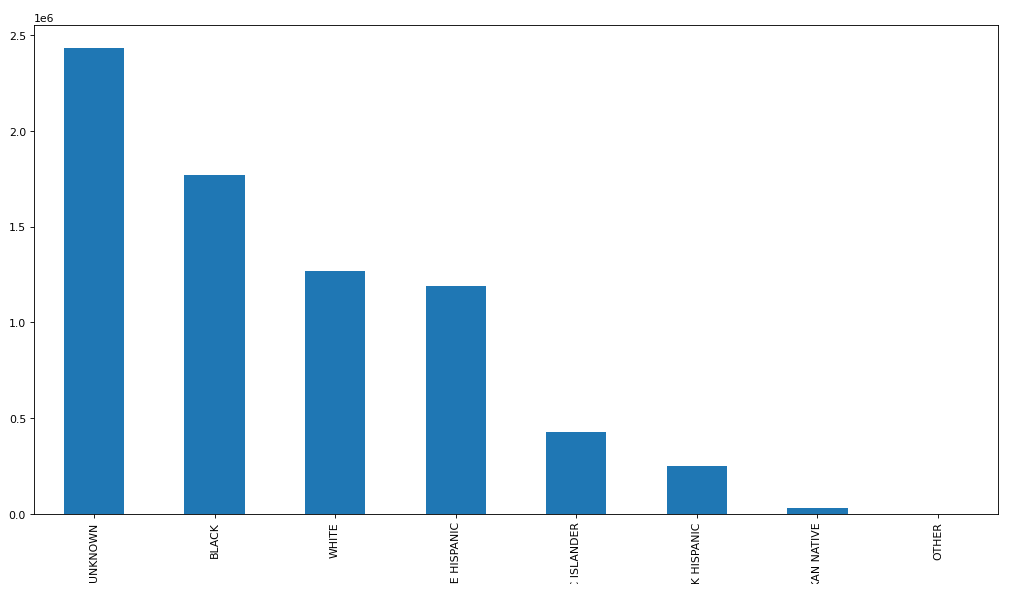
\includegraphics[width=0.85\textwidth]{img/hist_vic_race.png}
                    \caption{Histogram liczby zdarzeń dla danych ras poszkodowanych.}
                    \label{hist_vic_race}
                \end{figure}
                \begin{figure}[!htbp]
                    \centering
                    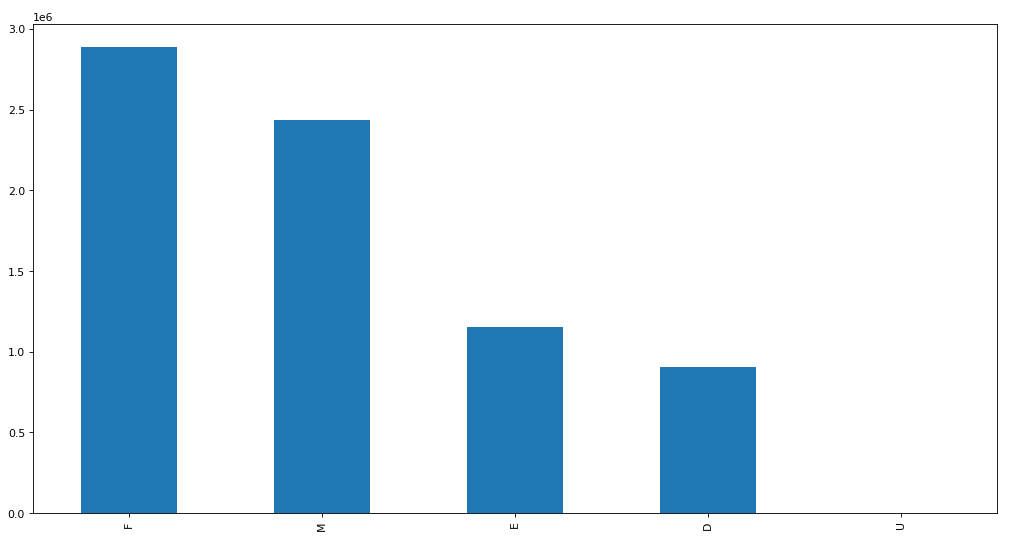
\includegraphics[width=0.85\textwidth]{img/hist_vic_sex.png}
                    \caption{Histogram liczby zdarzeń dla danych płci poszkodowanych.}
                    \label{hist_vic_sex}
                \end{figure}
                \FloatBarrier
                W przypadku cech ofiary/poszkodowanego sytuacja z grupami wiekowymi jest taka sama jak w przypadku cech podejrzanego. Rysunek \ref{hist_vic_age_group} pokazuje rozkład wieku ofiar po wstępnym oczyszczeniu zbioru. Również tutaj widać wyraźnie rozkład normalny. Rysunku \ref{hist_vic_race} oraz \ref{hist_vic_sex} pokazują, że wśród poszkodowanych najwięcej jest kobiet nieznanej rasy. Mamy tutaj do czynienia z dodatkowymi wartościami w kolumnie płci, które oznaczają grupy ludzi: instytucję lub państwo. Z powodu, że taki może być charakter poszkodowanych większość zdarzeń nie ma określonej płci poszkodowanego.
            }

            \subsubsection{Zależności między podejrzanym a ofiarą} {
                \begin{figure}[!htbp]
                    \centering
                    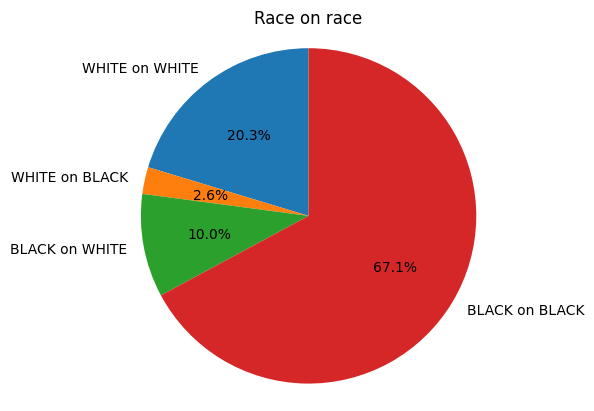
\includegraphics[width=0.75\textwidth]{img/3.2.8/Race#piechart-084518.png}
                    \caption{Wykres przedstawiający zależność pomiędzy podejrzanym a ofiarą, na podstawie ich rasy (uwzględnione zostały tylko dwie).}
                    \label{pie_chart_race}
                \end{figure}
                \begin{figure}[!htbp]
                    \centering
                    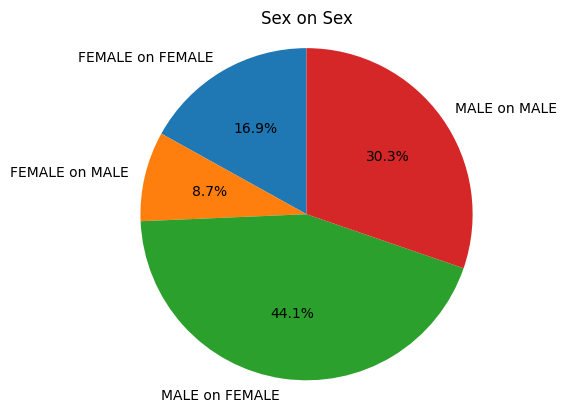
\includegraphics[width=0.75\textwidth]{img/3.2.8/Sex#piechart-084518.png}
                    \caption{Wykres przedstawiający zależność pomiędzy podejrzanym a ofiarą, na podstawie ich płci (uwzględnione zostały tylko dwie).}
                    \label{pie_chart_sex}
                \end{figure}
                \FloatBarrier

                Do wykresów \ref{pie_chart_race} i \ref{pie_chart_sex} zostały wybrane
                dwie rasy i płcie, które największą liczbę razy uczestniczyły w
                przestępstwie jako ofiara lub podejrzany. W ten sposób się
                zaobserwować, że największy odsetek przestępstw dotyczył tej samej
                rasy, można zatem stwierdzić, że odsetek przestępstw między rasowych
                jest niższy niż można było się spodziewać. Natomiast sprawdzenie
                rozkładu płci, nie zaskutkowało niespodziewanymi wnioskami. Mężczyźni
                ogólnie częściej są podejrzanymi o przestępstwa i częściej popełniają
                takie, w których ofiarami są kobiety niż mężczyźni.
            }
        }

    }
    
    \section{Ogólny schemat podjętego przetwarzania i analizy danych} {
        Ogólny schemat przetwarzania i analizy danych podjętych w tym zadaniu jest następujący:
        \begin{enumerate}
            \item Pozyskanie danych - pobranie na dysk ze źródła internetowego
            \item Przegląd danych i wstępna analiza statystyczna w celu rozeznania się w zawartości zbioru
            \item Rozważenie możliwych metod preprocessingu (czyszczenia danych, imputacji, kodowania kolumn, etc.)
            \item Dla każdego z wyznaczonych celów:
                \begin{enumerate}
                    \item Wstępne przetwarzanie danych (zależy od zastosowanych algorytmów i od realizowanego zadania)
                    \item Pierwszy eksperyment: uczenie modelu z wybranymi hiperparametrami
                    \item Dalsze eksperymenty: modyfikacja hiperparametrów i preprocessingu w zależności od uzyskanych wyników...
                    \item Wskazanie najlepszych wyników i wnioski z przeprowadzonych badań
                \end{enumerate}
        \end{enumerate}
    }
    \newpage

    \section{Cele projektu} \label{project_goals} {
        W ramach projektu sformułowane zostały trzy następujące cele.

        \subsection{Klasyfikacja rodzaju lub poziomu przestępstwa}
        \label{project_goal_1} {

            \subsubsection{Opis} {
                W ramach tego etapu przeprowadzony został szereg eksperymentów mających
                na celu stworzenie klasyfikatora typu przestępstwa (KY\_CD). W ramach porównania dokonano klasyfikacji poziomu wykroczenia,
                stanowiącego bardziej ogólną informacje. Podczas realizacji tego celu, pod uwagę zostały wzięte kolumny, przechowujące następujące informacje:
                \begin{itemize}
                    \item godzina zdarzenia
                    \item dzień tygodnia zdarzenia
                    \item odstęp między zgłoszeniem a zdarzeniem
                    \item czy doszło do skutku (CRM\_ATPT\_CPTD\_CD)
                    \item otoczenie zdarzenia
                    \item cechy podejrzanego
                    \item cechy ofiary
                    \item poziom lub typ przestępstwa w zależności od tego co klasyfikujemy
                \end{itemize}

                Wybrane cechy uległy drobnym modyfikacjom w trakcie trwania
                eksperymentów. 
                Z powodu małej liczby danych z dostępnymi informacjami o czasie trwania przestępstwa, pomysł wykorzystania tej danej został zarzucony.

                Informacja o dokładnej lokalizacji zdarzenia nie jest wykorzystana ze
narzędzia                względu na chęć stworzenia uniwersalnego narzędzia.

                Aby zrealizować zaproponowany cel wykorzystane zostały następujące metody:
                metody imputacji brakujących danych, prosta ekstrakcja cech (zwłaszcza z
                daty), naiwny klasyfikator Bayesa (ze względu na uzyskiwane wyniki w czasie trwania projektu, został porzucony) i lasy losowe (ze względu na uzyskiwane wyniki w czasie trwania projektu, metoda ta została potraktowana priorytetowo).

            }

            \subsubsection{Przygotowanie danych} {
                Bazując na założeniach celu oraz wiedzy, wyciągniętej z poprzednich checkpoint'ów, pod uwagę w czasie eksperymentów zostały brane pod uwagę następujące kolumny:
                \begin{itemize}
                    \item KY\_CD - kod popełnionego przestępstwa;
                    \item LAW\_CAT\_CD - poziom popełnionego przestępstwa;
                    \item CMPLNT\_FR\_DT - data zgłoszenia przestępstwa;
                    \item LOC\_OF\_OCCUR\_DESC - opis otoczenia zdarzenia;
                    \item SUSP\_AGE\_GROUP - Grupa wiekowa podejrzanego
                    \item SUSP\_RACE - Rasa podejrzanego
                    \item SUSP\_SEX - Płeć podejrzanego
                    \item VIC\_AGE\_GROUP - Grupa wiekowa ofiary
                    \item VIC\_RACE - Rasa ofiary
                    \item VIC\_SEX - Płeć ofiary
                \end{itemize}
                Powodem odrzucenia kolumny CRM\_ATPT\_CPTD\_CD było ogromne niezbalansowanie zawartych w niej danych. Dane poddano obróbce (preprocessing'owi), na którą składały się operacje różne w zależności od specyfiki przeprowadzanego eksperymentu. W celu redukcji wymiarów oraz ograniczenia liczby potencjalnych wartości, a co za tym idzie zmniejszenie liczby danych etykiet do kodowania (przetwarzanie dużego zbioru zakodowanych danych jest bardzo wymagającym wydajnościowo procesem, przy małym wpływie na jakość potencjalnych wyników) przeprowadzono następujące operacje grupowania:
                \begin{itemize}
                    \item grup wiekowych, tak aby można było nadać im odpowiednią etykietę ("<18", "18-24", "25-44", "45-64", "65+", "UNKNOWN") oraz jej ewentualna imputacja  najczęściej występującą wartością;
                    \item rasy (podejrzanego i ofiary), tak aby można było nadać im odpowiednią etykietę (zależną od eksperymentu) - ["WHITE", "BLACK", "HISPANIC", "UNKNOWN", "OTHER"], lub ["WHITE", "BLACK", "HISPANIC", "UNKNOWN", "OTHER"]
                    \item (podejrzanego i ofiary), tak aby można było nadać im odpowiednią etykietę  - ["MALE", "FEMALE", "OTHER"];
                    \item pozycji otoczenia zdarzenia, tak aby można było nadać im odpowiednią etykietę  - ["UNKNOWN", "FRONT OF", "INSIDE", "OTHER"];
                \end{itemize}
                Po dokonaniu grupowania, ze zbioru zostały usunięte te wiersze, dla których wykorzystywane w eksperymentach wartości były puste. Następnie (w przypadku eksperymentów, w których było to badane) obróbce poddana została informacja o dacie zgłoszenia przestępstwa. W pierwszym kroku wyekstrahowano z tej kolumny informacje o dniu tygodnia i dniu roku. Następnie, aby nie stracić potencjalnie przydatnej informacji, jaką niesie cykliczność dni tygodnia, czy też roku, obie te wartości zostały zapisane przy pomocy odpowiadających sobie wartości funkcji trygonometrycznych sinus i cosinus.
                Ostatnim krokiem przygotowania danych było odpowiednie zakodowanie danych kolumn, w zależności od tego jaki typ danych prezentowały.
            }

            \subsubsection{Przetwarzanie i analiza danych} {
                Na wstępie przeprowadzono serię eksperymentów, w trakcie których określano najoptymalniejszy dobór cech do klasyfikacji w oparciu o dokładność klasyfikacji oraz wskazania ważności cech (ang. \textit{feature importance}). W tym celu wykorzystano dwie przeciwstawne metody, dzięki czemu można było uzyskać pełniejszy obraz (zmniejszone zostało prawdopodobieństwo podatności któreś metody, na np. dane kategorialne), wykorzystano:
                \begin{itemize}
                    \item metodę opartą o \textit{mean decrease in impurity};
                    \item metodę opartą o \textit{feature permutation}
                \end{itemize}
                
                Eksperymenty, mające na celu wyodrębnienie najważniejszych cel, zostały przeprowadzone na wycinku zbioru danych - dla 100000 wierszy danych. W tych eksperymentach były generowane pary wykresów (rezultaty działania dwóch wspomnianych metod badania ważności cech) dla klasyfikacji kodu przestępstwa (\textit{key-code}) oraz poziomu wykroczenia (\textit{law-breaking-level}), natomiast zamieszczano je w komplecie, tylko w sytuacji gdy różniły się od siebie w sposób znaczący i warty analizy, w przeciwnym razie zostały one w sprawozdaniu pominięte. Dodatkowo zaprezentowane zostaną tabelę z informacją o dokładności klasyfikacji, wraz z porównaniem do ostatnio przeprowadzonego eksperymentu.
                \paragraph{Eksperyment nr 1}{
                    W tym eksperymencie pogrupowano rasy pogrupowano zgodnie z kategoriami ["WHITE", "BLACK", "HISPANIC", "UNKNOWN", "OTHER"] oraz wykorzystano dzień tygodnia i dzień roku (w postaci par wartości funkcji sinus i cosinus).
                    \begin{figure}[!htbp]
                        \centering
                        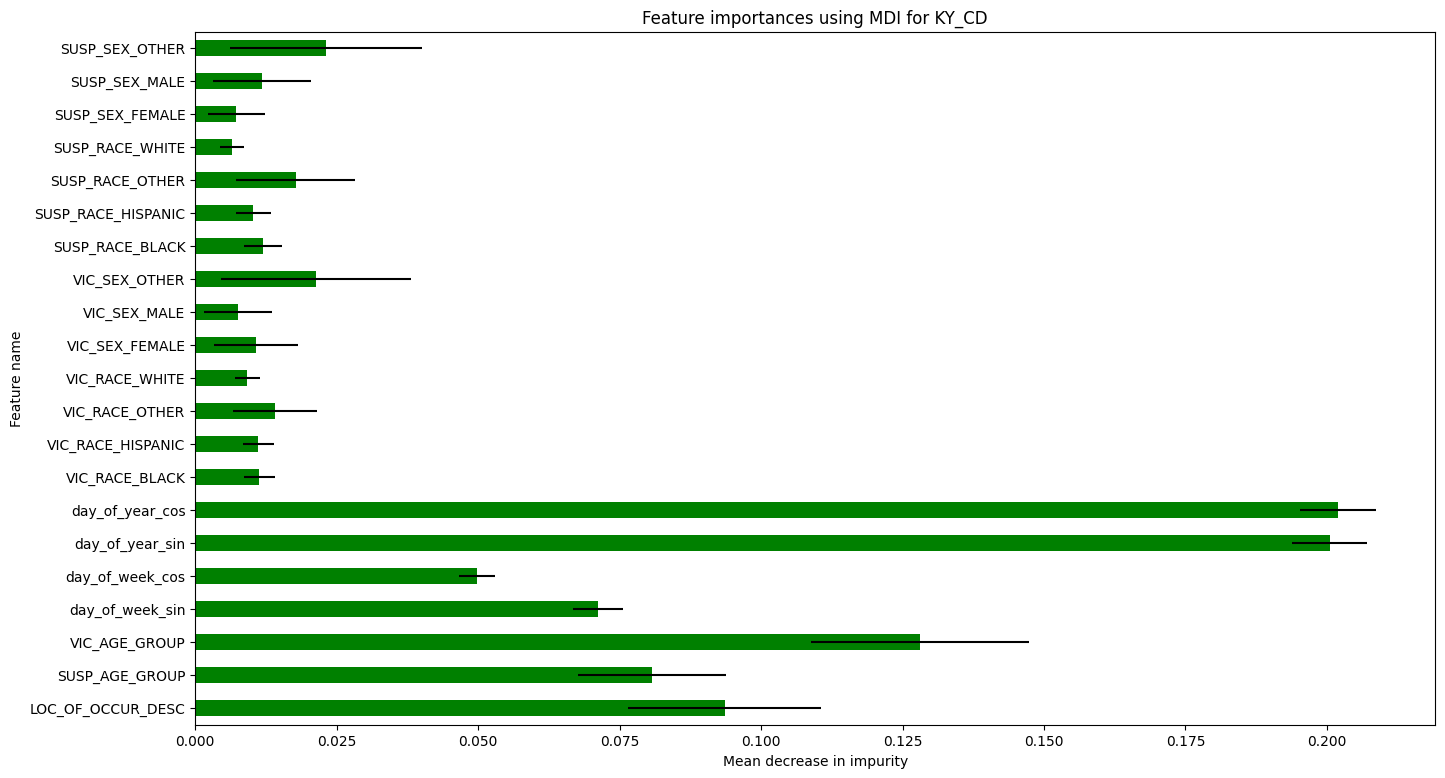
\includegraphics[width=0.9\textwidth]{img/5.1.3/1/Feature importances using MDI for KY_CD.png}
                        \caption{Feature importances (MDI), w klasyfikacji key-code}
                        \label{goal_1_exp_1_imp_mdi_key}
                    \end{figure}
                    
                    \begin{figure}[!htbp]
                        \centering
                        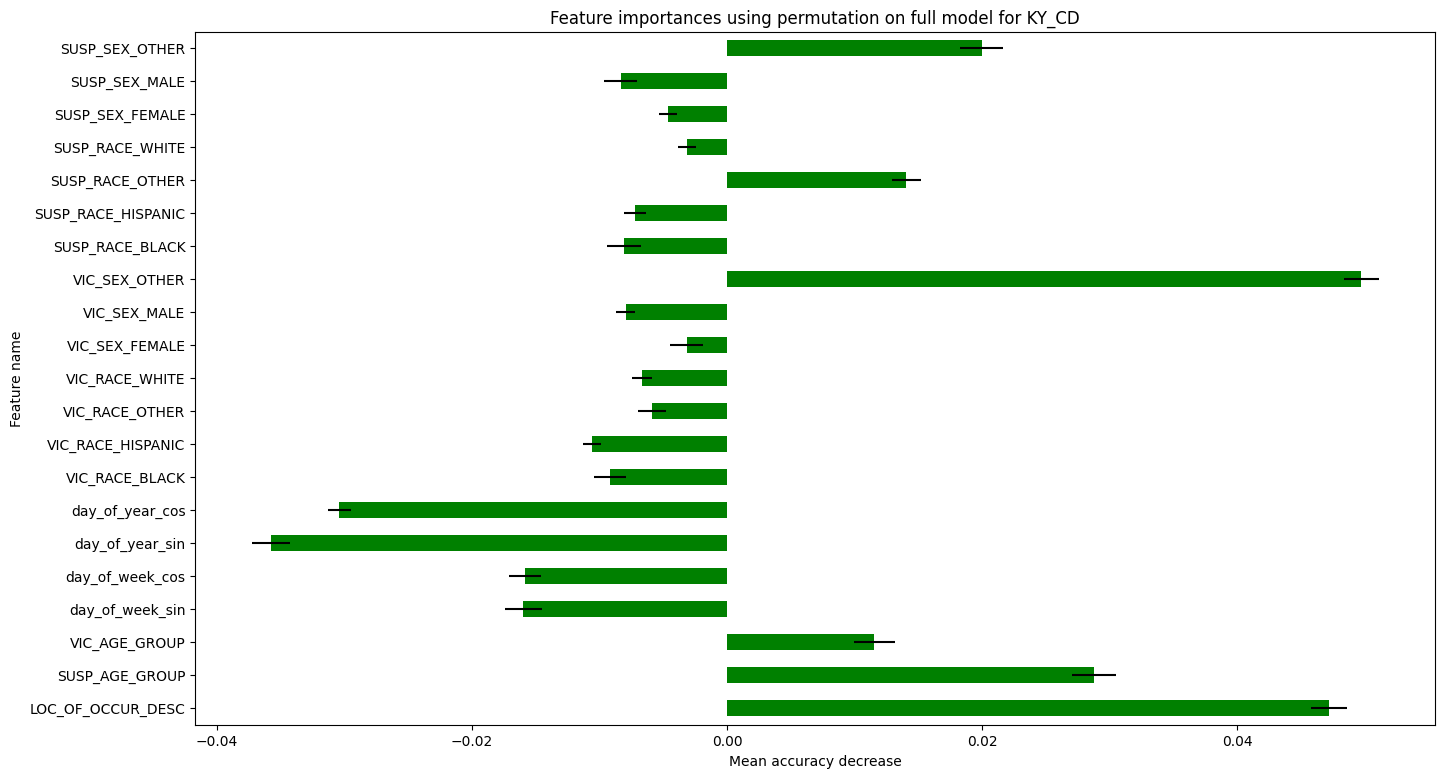
\includegraphics[width=0.9\textwidth]{img/5.1.3/1/Feature importances using permutation on full model for KY_CD.png}
                        \caption{Feature importances (permutation), w klasyfikacji key-code}
                        \label{goal_1_exp_1_imp_perm_key}
                    \end{figure}
                    
                    \begin{table}
                    \centering
                     \begin{tabular}{|c|c|c|c|}
                            \hline
                          Nazwa metryki & Wartość & Zmiana wartości & Klasyfikacja \\ \hline
                            Accuracy &  29,605\% & 0 & key-code\\ \hline
                            Accuracy &  50,9\% & 0 & law-breaking-level\\ \hline
                        \end{tabular}
                        \caption{Wyniki dla eksperymentu nr 1}
                        \label{goal_1_exp_1_results}
                     \end{table}
                     \FloatBarrier
                     
                     Warto zwrócić uwagę na dużą rozbieżność dotyczącą przydatności cech według algorytmów (wykresy \ref{goal_1_exp_1_imp_mdi_key} i \ref{goal_1_exp_1_imp_perm_key}), w kontekście daty zgłoszenia zdarzenia, zostało to uwzględnione w kolejnym eksperymencie.
                }
                \paragraph{Eksperyment nr 2}{
                    W tym eksperymencie pogrupowano rasy pogrupowano zgodnie z kategoriami ["WHITE", "BLACK", "HISPANIC", "UNKNOWN", "OTHER"], natomiast nie wykorzystano dnia tygodnia i dnia roku.
                    \begin{figure}[!htbp]
                        \centering
                        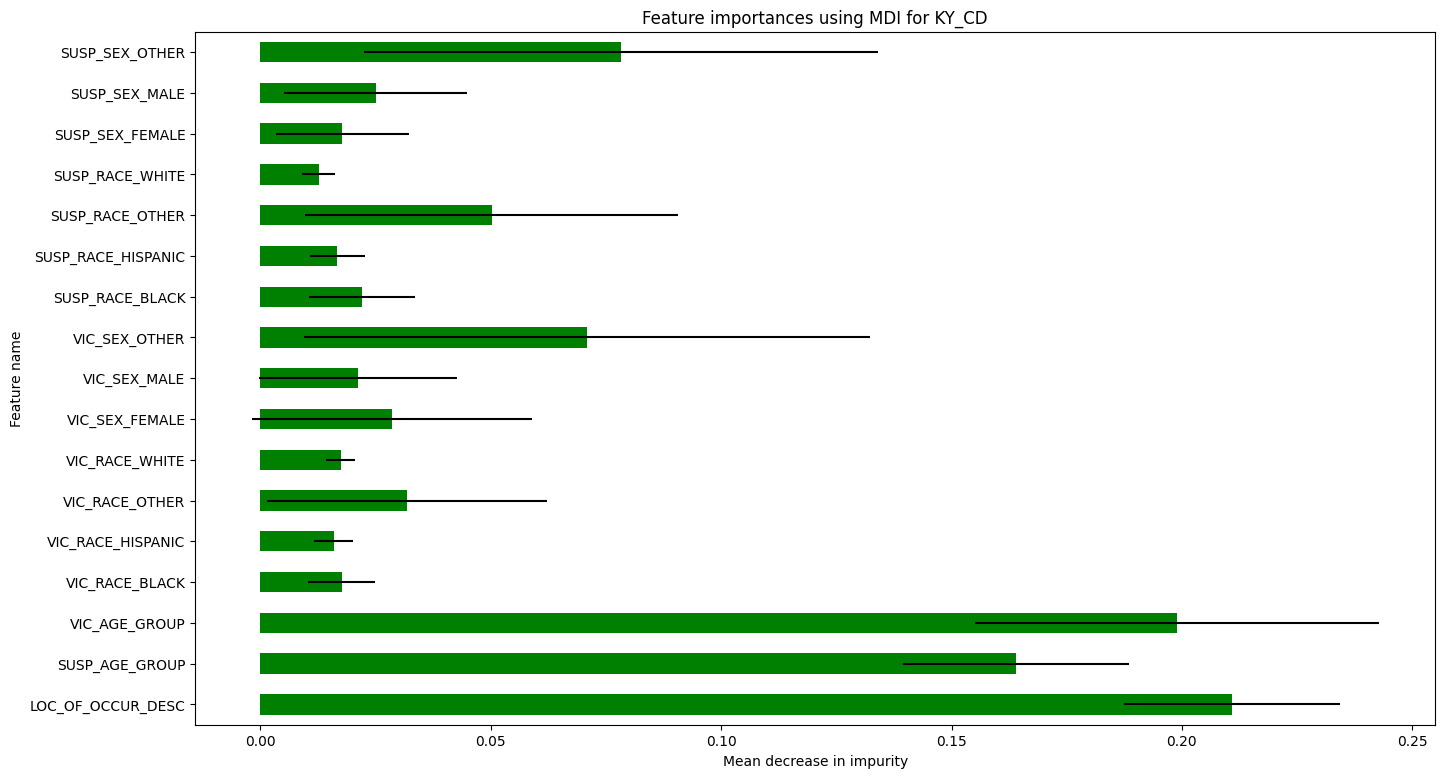
\includegraphics[width=0.9\textwidth]{img/5.1.3/2/Feature importances using MDI for KY_CD.png}
                        \caption{Feature importances (MDI), w klasyfikacji key-code}
                        \label{goal_1_exp_2_imp_mdi_key}
                    \end{figure}
                    
                    \begin{figure}[!htbp]
                        \centering
                        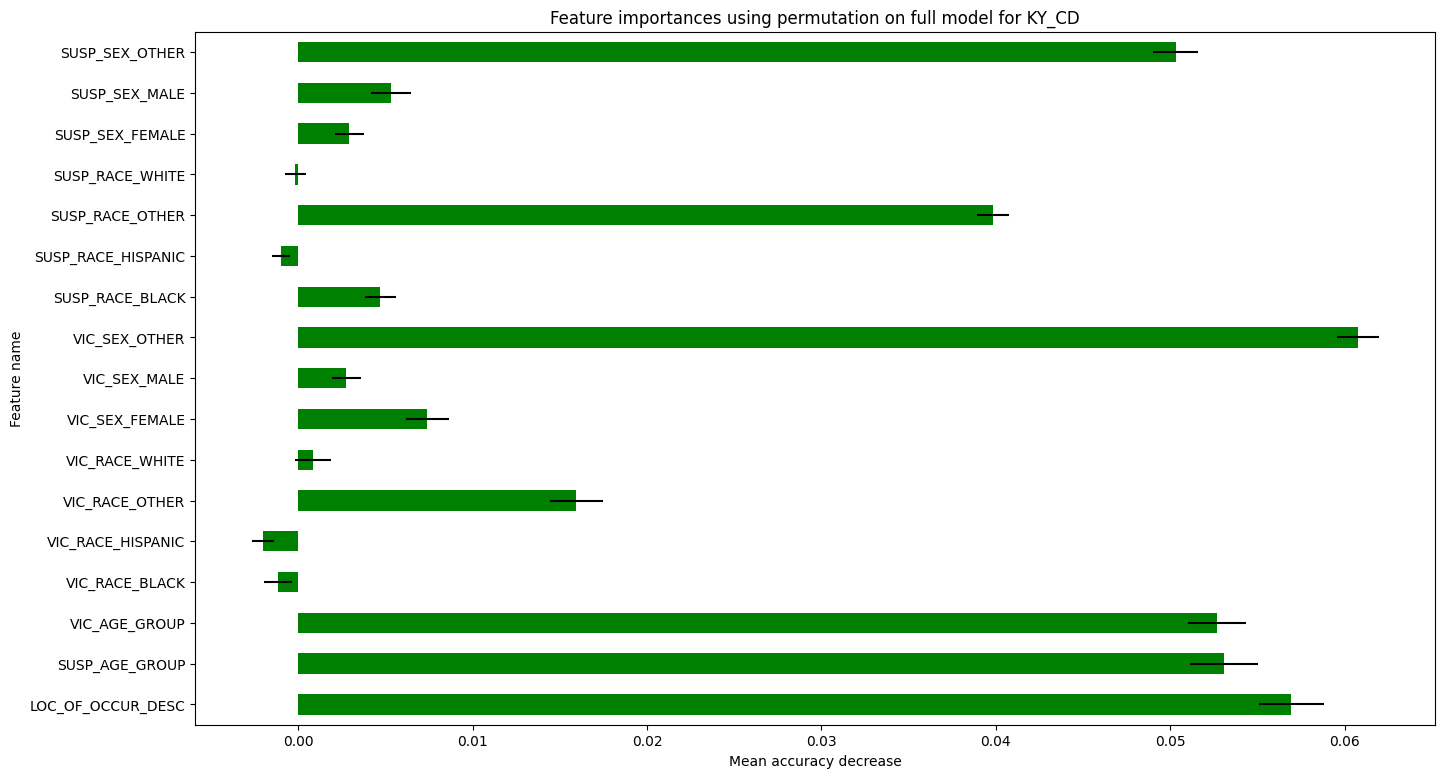
\includegraphics[width=0.9\textwidth]{img/5.1.3/2/Feature importances using permutation on full model for KY_CD.png}
                        \caption{Feature importances (permutation), w klasyfikacji key-code}
                        \label{goal_1_exp_2_imp_perm_key}
                    \end{figure}
                    
                    \begin{table}
                    \centering
                     \begin{tabular}{|c|c|c|c|}
                            \hline
                          Nazwa metryki & Wartość & Zmiana wartości & Klasyfikacja \\ \hline
                            Accuracy &  34,815\% & +5,21 & key-code\\ \hline
                            Accuracy &  54,0\% & +3,1 & law-breaking-level\\ \hline
                        \end{tabular}
                        \caption{Wyniki dla eksperymentu nr 2}
                        \label{goal_1_exp_2_results}
                     \end{table}
                     \FloatBarrier
                     
                     Na podstawie wzrostów dokładności klasyfikacji dla obu cech, widocznych w tabeli \ref{goal_1_exp_2_results}, decyzję o nie wykorzystaniu daty należy uznać za korzystną. Po analizie danych na wykresach \ref{goal_1_exp_2_imp_mdi_key} i \ref{goal_1_exp_2_imp_perm_key} zmienione zostaną etykiety ras, tak aby nie wykorzystywać jednej z obecnych - "HISPANIC".
                }
                \paragraph{Eksperyment nr 3}{
                    W tym eksperymencie pogrupowano rasy pogrupowano zgodnie z kategoriami ["WHITE", "BLACK", "UNKNOWN", "OTHER"].
                    \begin{figure}[!htbp]
                        \centering
                        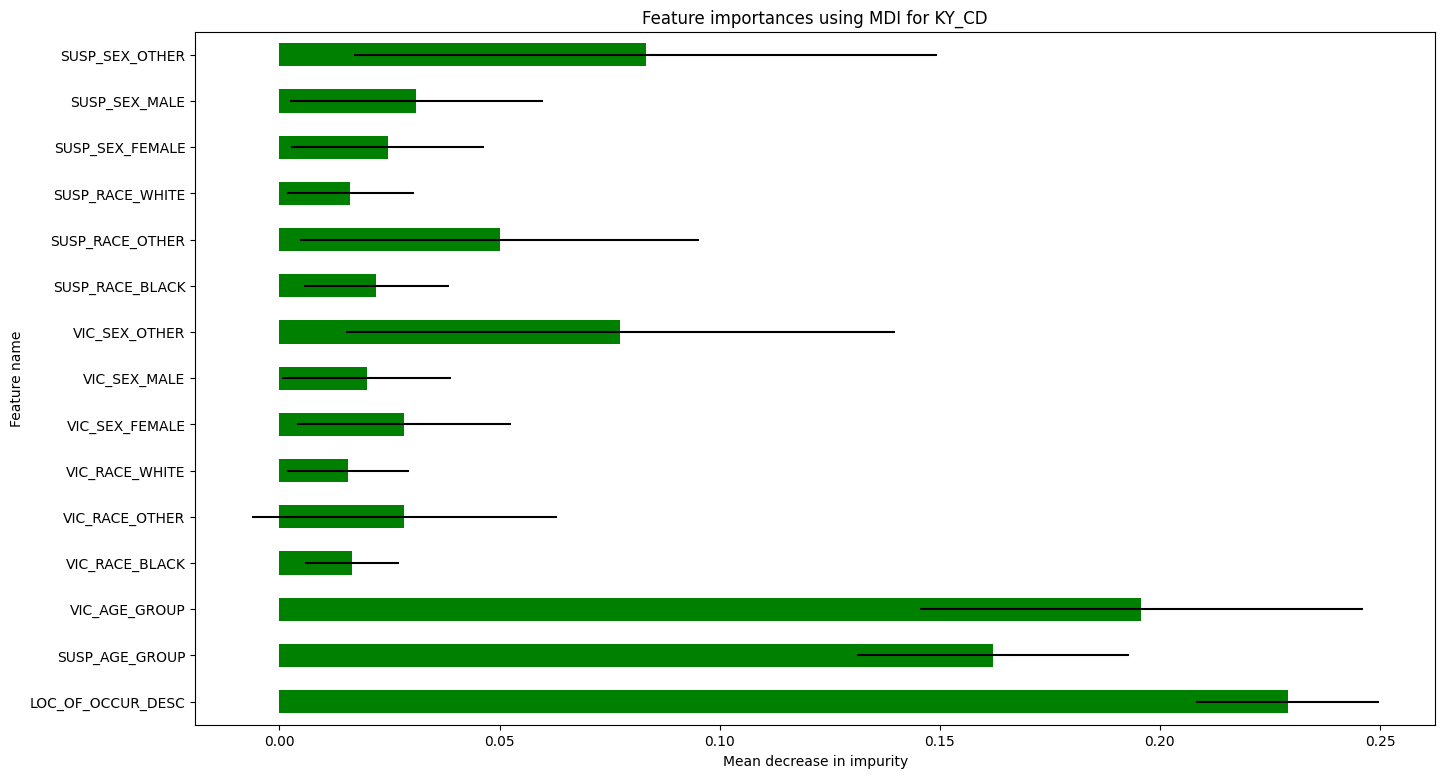
\includegraphics[width=0.9\textwidth]{img/5.1.3/3/Feature importances using MDI for KY_CD.png}
                        \caption{Feature importances (MDI), w klasyfikacji key-code}
                        \label{goal_1_exp_3_imp_mdi_key}
                    \end{figure}
                    
                    \begin{figure}[!htbp]
                        \centering
                        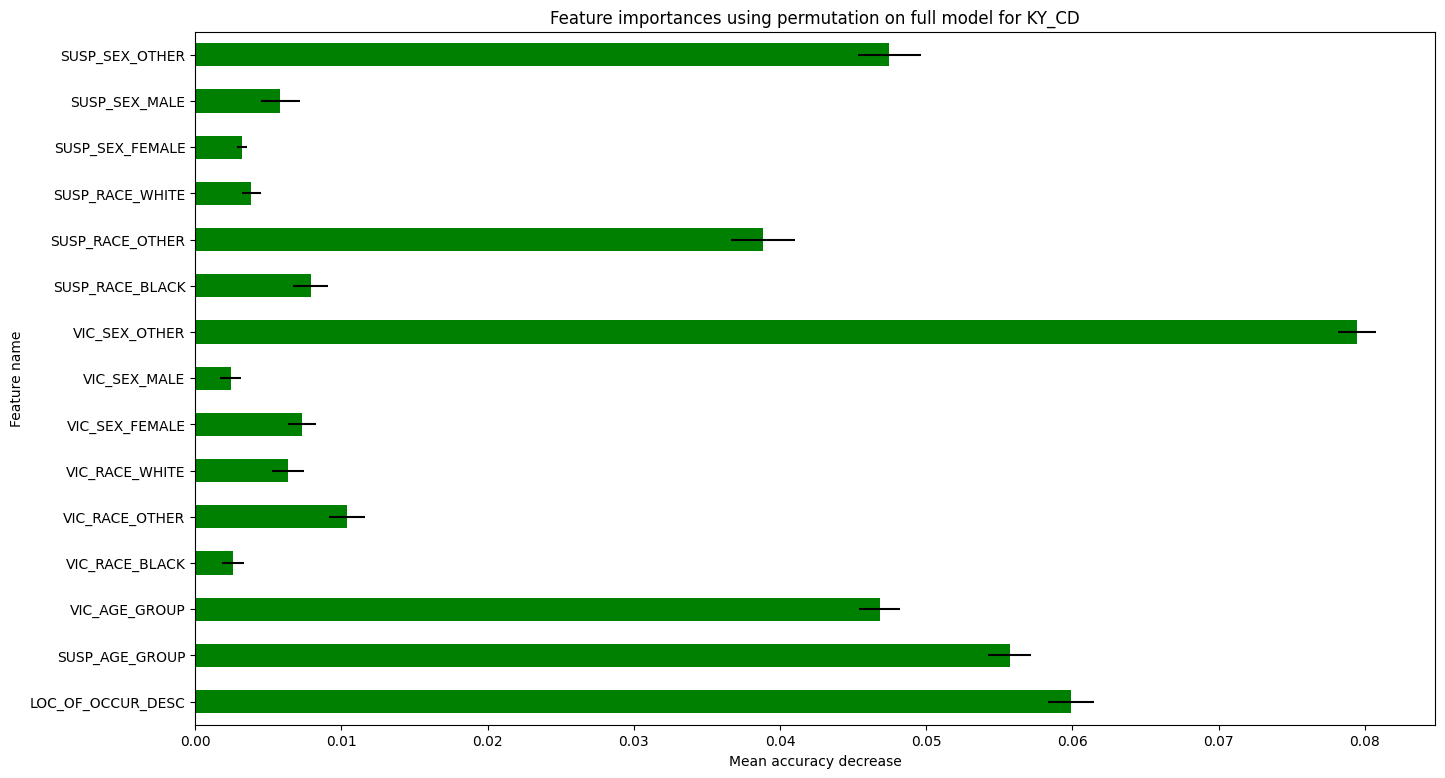
\includegraphics[width=0.9\textwidth]{img/5.1.3/3/Feature importances using permutation on full model for KY_CD.png}
                        \caption{Feature importances (permutation), w klasyfikacji key-code}
                        \label{goal_1_exp_3_imp_perm_key}
                    \end{figure}
                    
                    \begin{table}
                    \centering
                     \begin{tabular}{|c|c|c|c|}
                            \hline
                          Nazwa metryki & Wartość & Zmiana wartości & Klasyfikacja \\ \hline
                            Accuracy &  35,275\% & +0,46 & key-code\\ \hline
                            Accuracy &  54,245\% & +0,245 & law-breaking-level\\ \hline
                        \end{tabular}
                        \caption{Wyniki dla eksperymentu nr 3}
                        \label{goal_1_exp_3_results}
                     \end{table}
                     \FloatBarrier
                     Na podstawie wzrostów dokładności klasyfikacji dla obu cech, widocznych w tabeli \ref{goal_1_exp_3_results}, decyzję o zmianie sposobu grupowania ras należy uznać za korzystną.
                }
                \paragraph{Eksperyment nr 4}{
                    W tym eksperymencie, w oparciu o poprzednie eksperymenty zmieniono podejście do przechowywania informacji o rasie podejrzanego i ofiary. Postanowiono wykorzystać zależność pomiędzy ofiarą a podejrzanym, zaprezentowaną na wykresie \ref{pie_chart_race}.
                    \begin{figure}[!htbp]
                        \centering
                        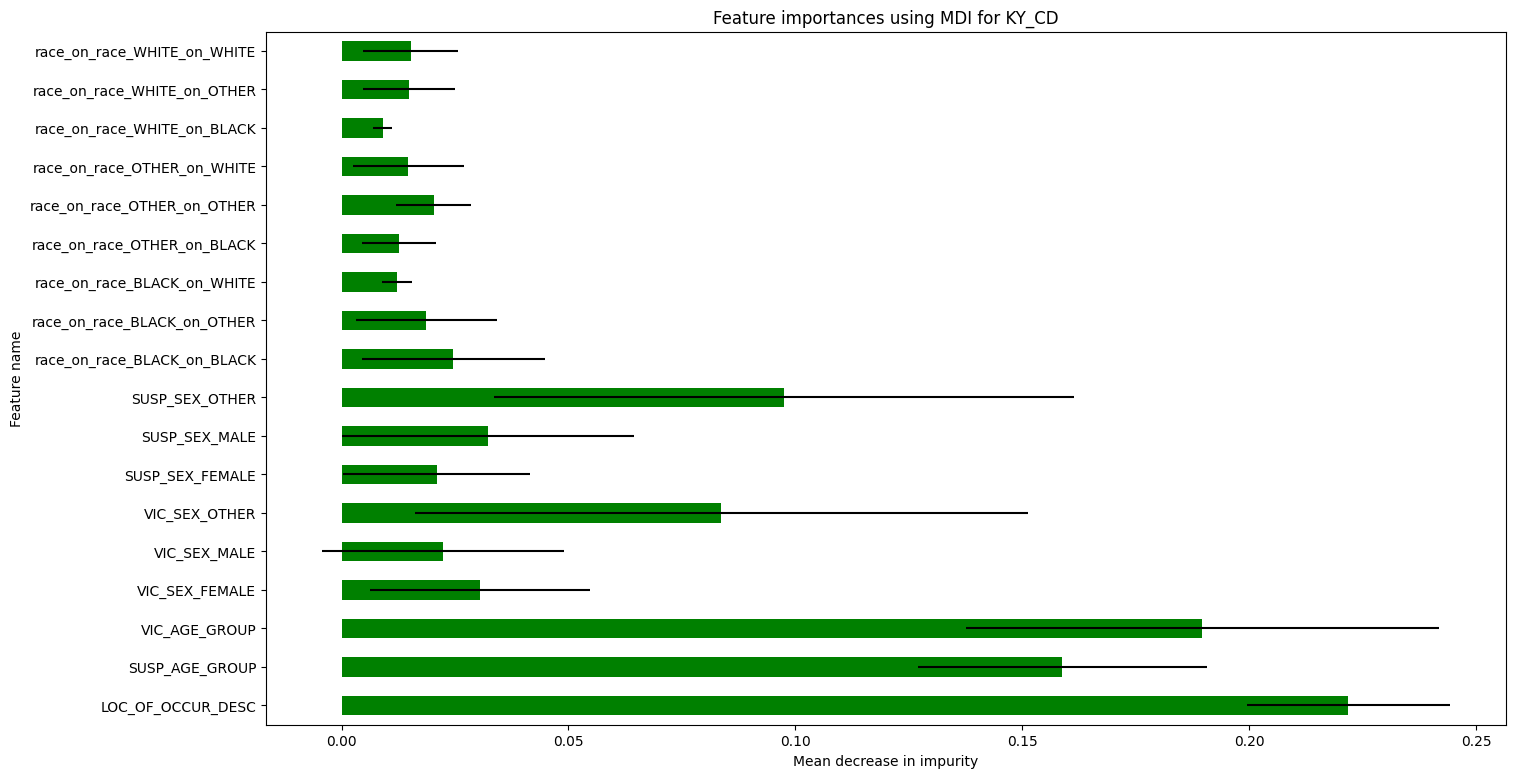
\includegraphics[width=0.9\textwidth]{img/5.1.3/4/Feature importances using MDI for KY_CD.png}
                        \caption{Feature importances (MDI), w klasyfikacji key-code}
                        \label{goal_1_exp_4_imp_mdi_key}
                    \end{figure}
                    
                    \begin{figure}[!htbp]
                        \centering
                        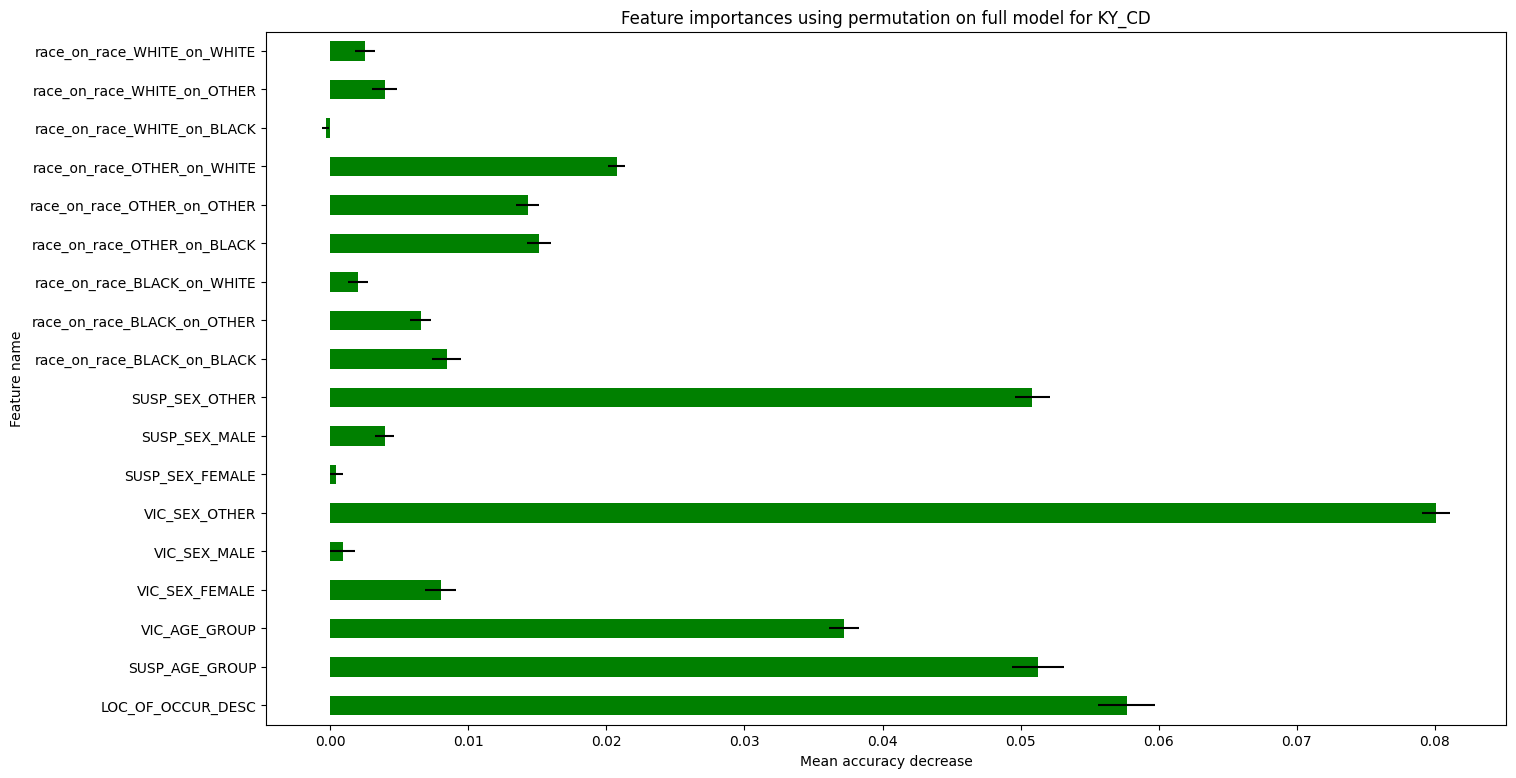
\includegraphics[width=0.9\textwidth]{img/5.1.3/4/Feature importances using permutation on full model for KY_CD.png}
                        \caption{Feature importances (permutation), w klasyfikacji key-code}
                        \label{goal_1_exp_4_imp_perm_key}
                    \end{figure}
                    
                    \begin{figure}[!htbp]
                        \centering
                        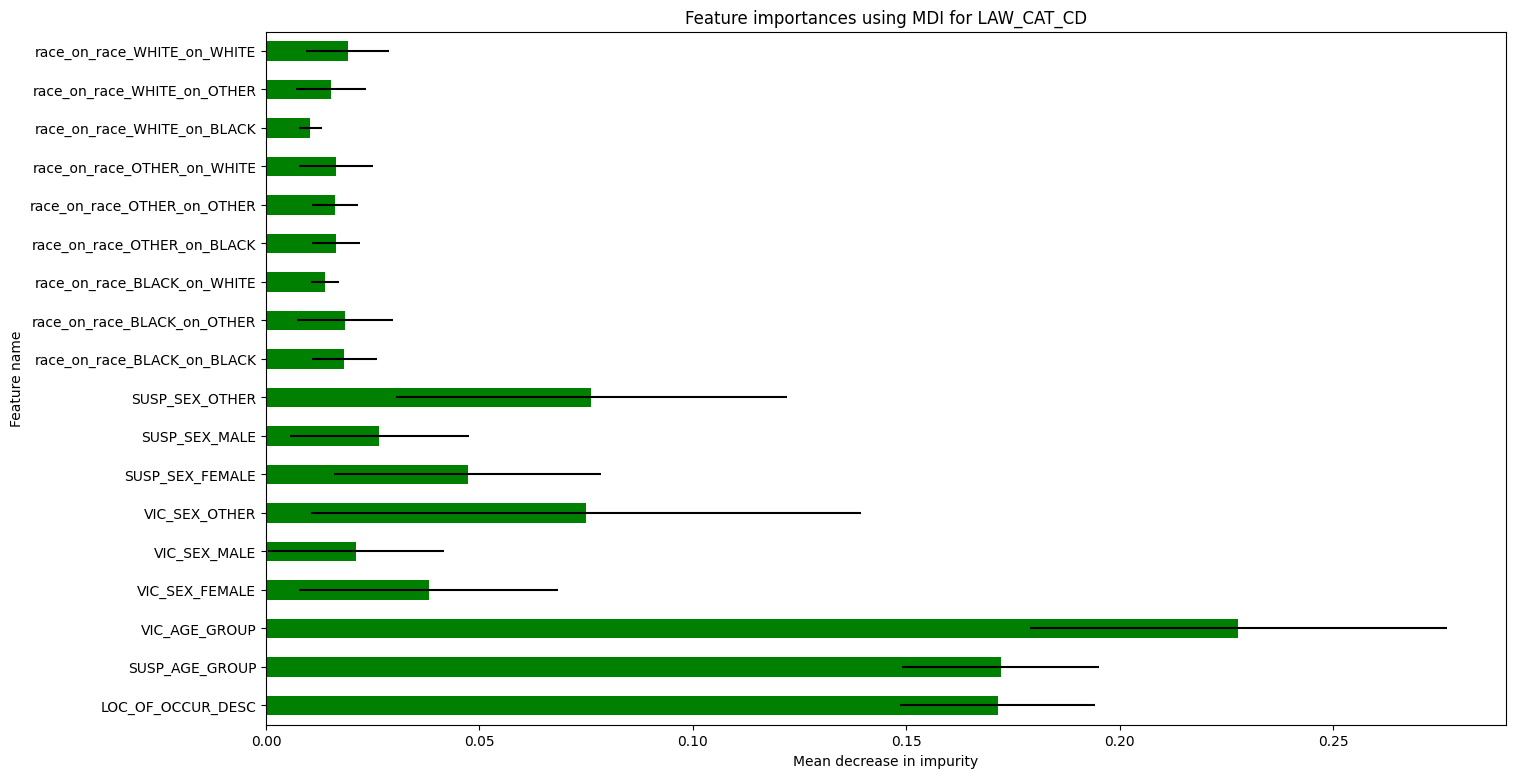
\includegraphics[width=0.9\textwidth]{img/5.1.3/4/Feature importances using MDI for LAW_CAT_CD.png}
                        \caption{Feature importances (MDI), w klasyfikacji law-breaking-level}
                        \label{goal_1_exp_4_imp_mdi_law}
                    \end{figure}
                    
                    \begin{figure}[!htbp]
                        \centering
                        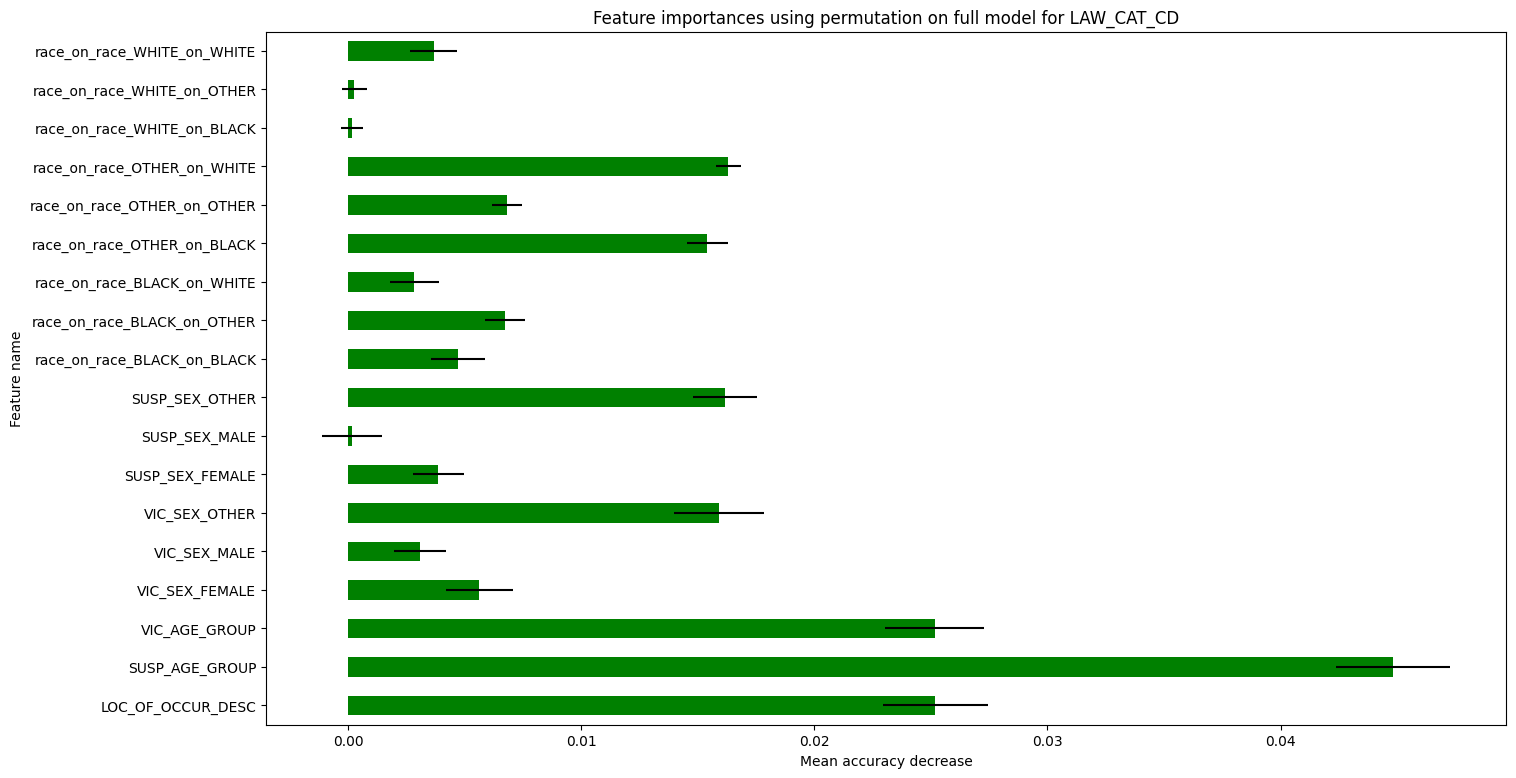
\includegraphics[width=0.9\textwidth]{img/5.1.3/4/Feature importances using permutation on full model for LAW_CAT_CD.png}
                        \caption{Feature importances (permutation), w klasyfikacji law-breaking-level}
                        \label{goal_1_exp_4_imp_perm_law}
                    \end{figure}
                    
                    \begin{table}
                    \centering
                     \begin{tabular}{|c|c|c|c|}
                            \hline
                          Nazwa metryki & Wartość & Zmiana wartości & Klasyfikacja \\ \hline
                            Accuracy &  35,0\% & -0,275 & key-code\\ \hline
                            Accuracy &  53,71\% & -0,535 & law-breaking-level\\ \hline
                        \end{tabular}
                        \caption{Wyniki dla eksperymentu nr 4}
                        \label{goal_1_exp_4_results}
                     \end{table}
                     \FloatBarrier
                     Na podstawie spadków dokładności klasyfikacji dla obu cech, widocznych w tabeli \ref{goal_1_exp_4_results}, decyzję o zmianie sposobu grupowania ras należy uznać za niekorzystną. Jednak wykresy \ref{goal_1_exp_4_imp_mdi_key}, \ref{goal_1_exp_4_imp_mdi_law}, \ref{goal_1_exp_4_imp_perm_key}, \ref{goal_1_exp_4_imp_perm_law}, skłaniają do pomysłu aby podobnej modyfikacji poddać płeć.
                }
                \paragraph{Eksperyment nr 5}{
                    W tym eksperymencie, postanowiono nie modyfikować sposobu przechowywanie informacji o rasie podejrzanego i ofiary. Wykorzystano natomiast zależność pomiędzy ofiarą a podejrzanym, zaprezentowaną na wykresie \ref{pie_chart_sex} i zmieniomo sposób przechowywania płci.
                    \begin{figure}[!htbp]
                        \centering
                        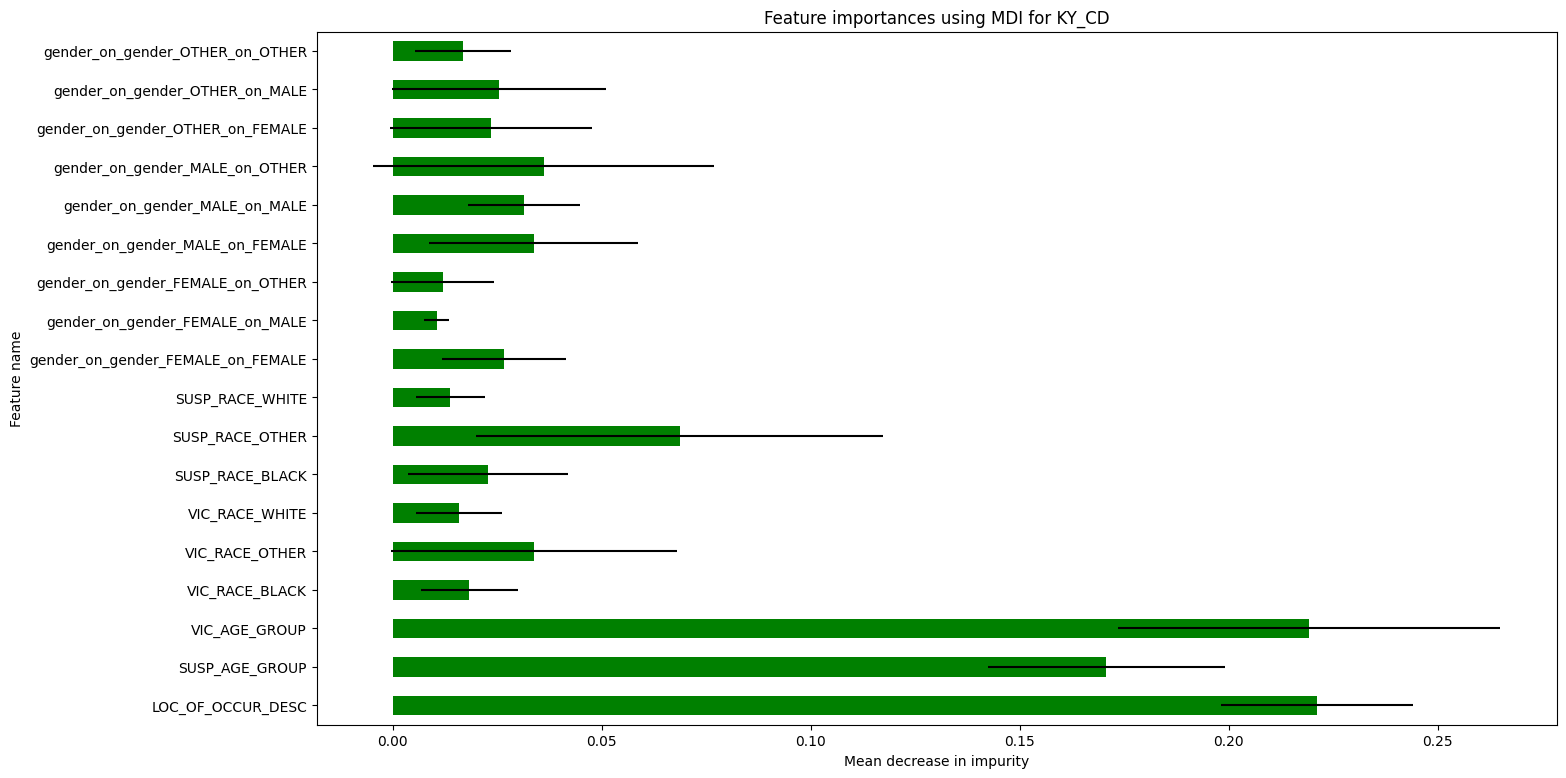
\includegraphics[width=\textwidth]{img/5.1.3/5/Feature importances using MDI for KY_CD.png}
                        \caption{Feature importances (MDI), w klasyfikacji key-code}
                        \label{goal_1_exp_5_imp_mdi_key}
                    \end{figure}
                    
                    \begin{figure}[!htbp]
                        \centering
                        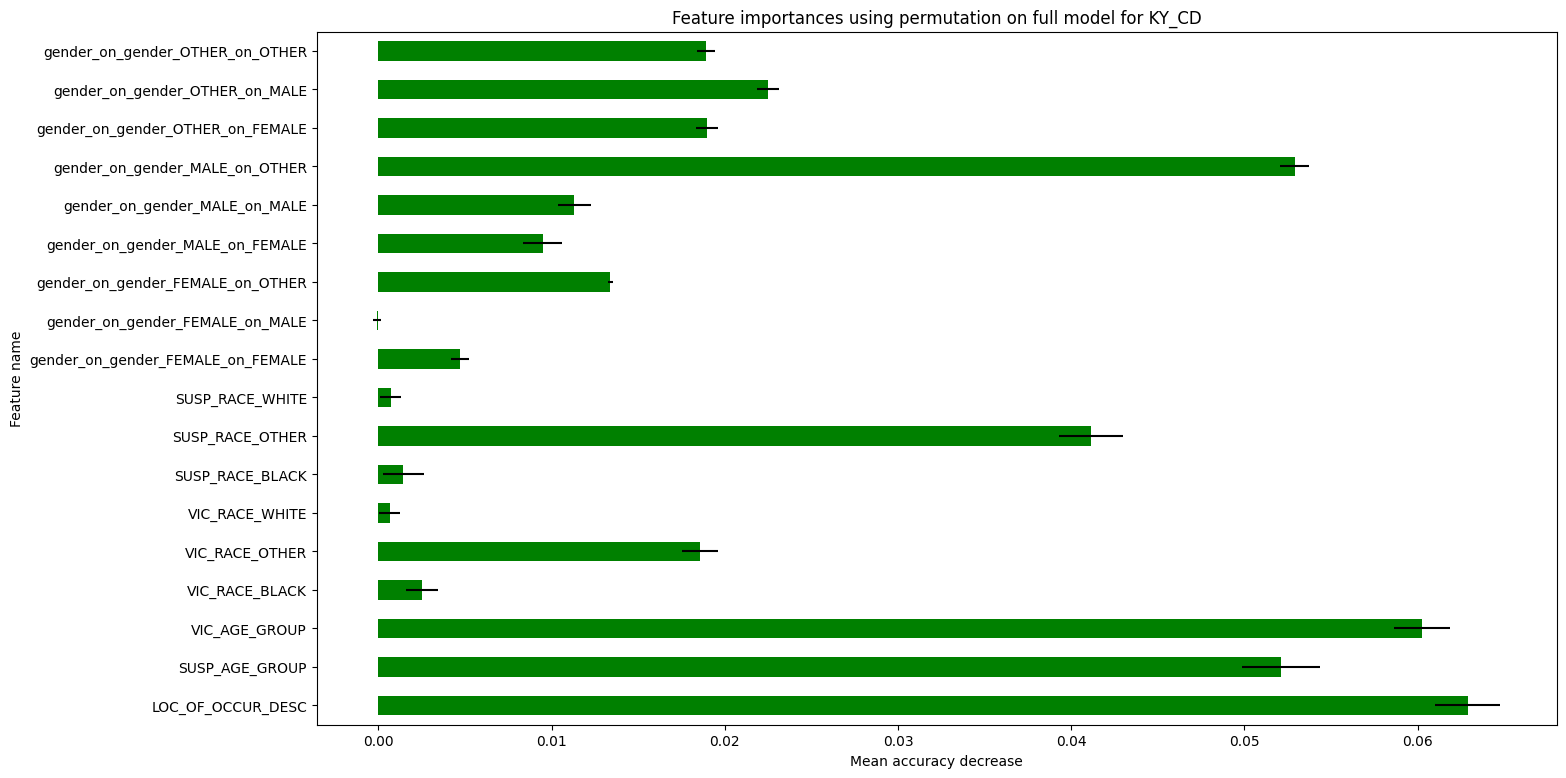
\includegraphics[width=\textwidth]{img/5.1.3/5/Feature importances using permutation on full model for KY_CD.png}
                        \caption{Feature importances (permutation), w klasyfikacji key-code}
                        \label{goal_1_exp_5_imp_perm_key}
                    \end{figure}
                    
                    \begin{figure}[!htbp]
                        \centering
                        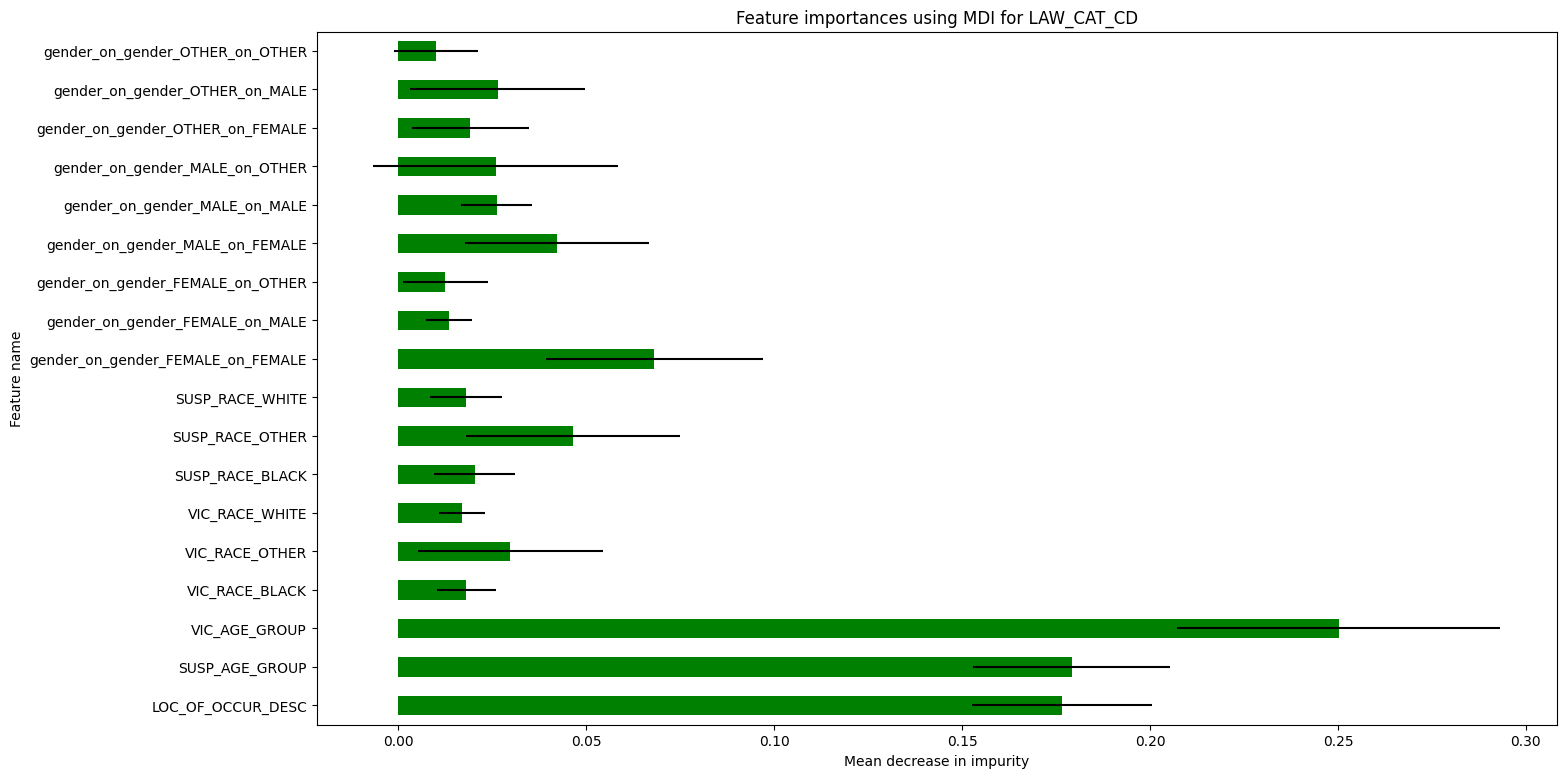
\includegraphics[width=\textwidth]{img/5.1.3/5/Feature importances using MDI for LAW_CAT_CD.png}
                        \caption{Feature importances (MDI), w klasyfikacji law-breaking-level}
                        \label{goal_1_exp_5_imp_mdi_law}
                    \end{figure}
                    
                    \begin{figure}[!htbp]
                        \centering
                        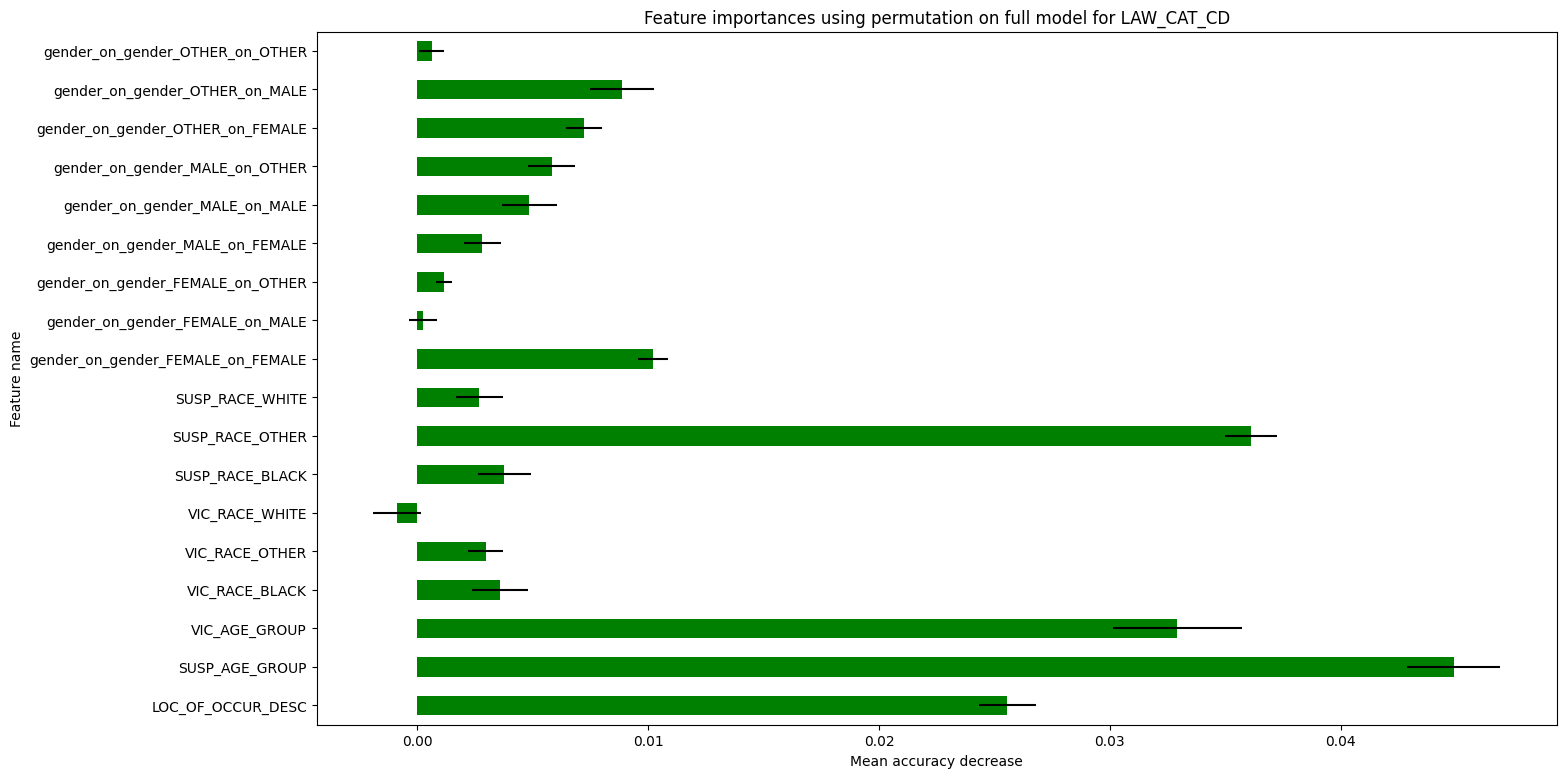
\includegraphics[width=\textwidth]{img/5.1.3/5/Feature importances using permutation on full model for LAW_CAT_CD.png}
                        \caption{Feature importances (permutation), w klasyfikacji law-breaking-level}
                        \label{goal_1_exp_5_imp_perm_law}
                    \end{figure}
                    
                    \begin{table}
                    \centering
                     \begin{tabular}{|c|c|c|c|}
                            \hline
                          Nazwa metryki & Wartość & Zmiana wartości & Klasyfikacja \\ \hline
                            Accuracy &  35,325\% & +0,325 & key-code\\ \hline
                            Accuracy &  53,575\% & -0,135 & law-breaking-level\\ \hline
                        \end{tabular}
                        \caption{Wyniki dla eksperymentu nr 5}
                        \label{goal_1_exp_5_results}
                     \end{table}
                     \FloatBarrier
                }
            
                    \paragraph{Eksperyment nr 6}{
                    W tym eksperymencie, postanowiono sprawdzić zachowanie klasyfikacji przy zmienionym sposobie przechowywania informacji zarówno o rasie jak i o płci.
                    \begin{figure}[!htbp]
                        \centering
                        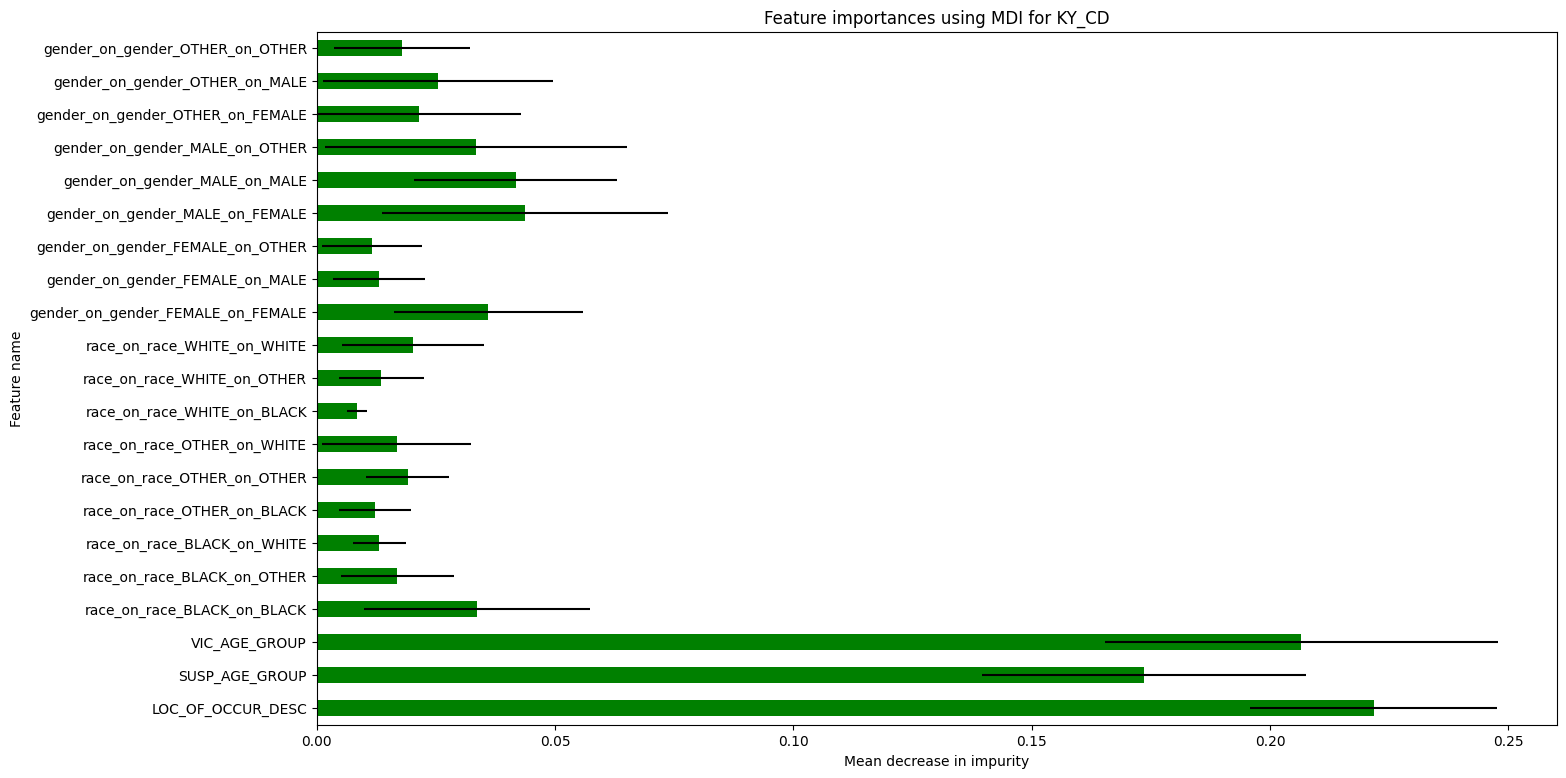
\includegraphics[width=\textwidth]{img/5.1.3/6/Feature importances using MDI for KY_CD.png}
                        \caption{Feature importances (MDI), w klasyfikacji key-code}
                        \label{goal_1_exp_6_imp_mdi_key}
                    \end{figure}
                    
                    \begin{figure}[!htbp]
                        \centering
                        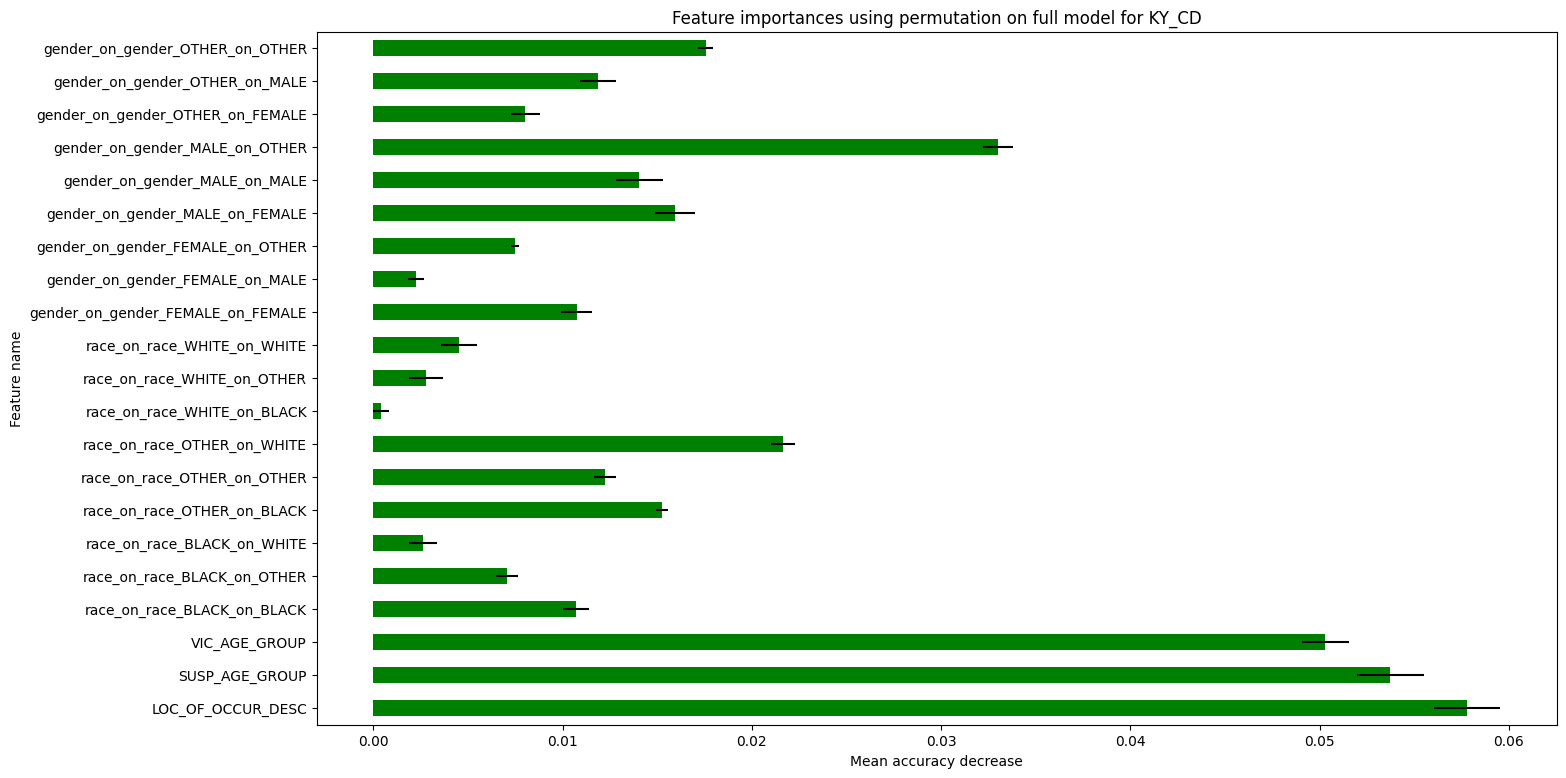
\includegraphics[width=\textwidth]{img/5.1.3/6/Feature importances using permutation on full model for KY_CD.png}
                        \caption{Feature importances (permutation), w klasyfikacji key-code}
                        \label{goal_1_exp_6_imp_perm_key}
                    \end{figure}
                    
                    \begin{figure}[!htbp]
                        \centering
                        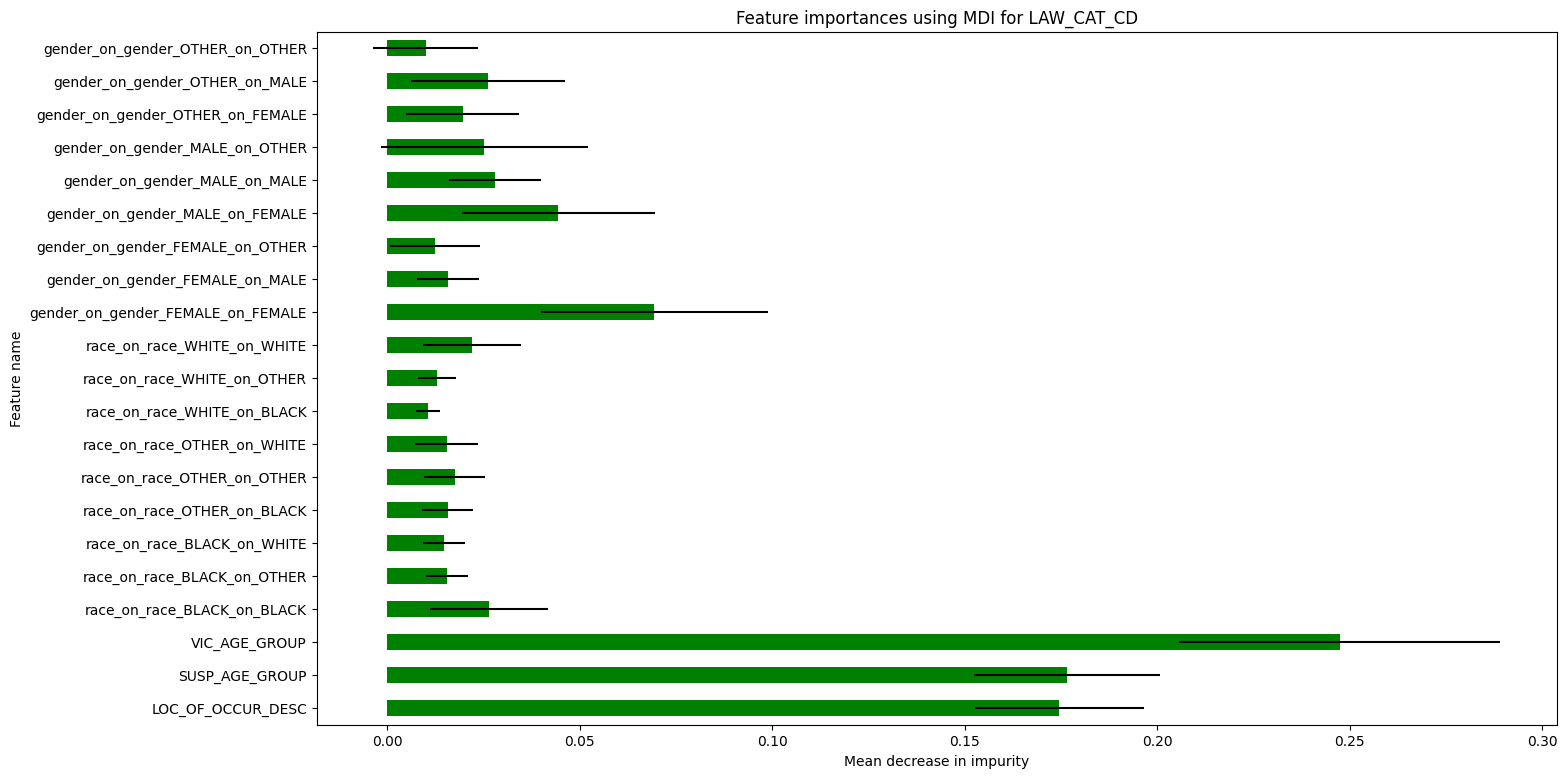
\includegraphics[width=\textwidth]{img/5.1.3/6/Feature importances using MDI for LAW_CAT_CD.png}
                        \caption{Feature importances (MDI), w klasyfikacji law-breaking-level}
                        \label{goal_1_exp_6_imp_mdi_law}
                    \end{figure}
                    
                    \begin{figure}[!htbp]
                        \centering
                        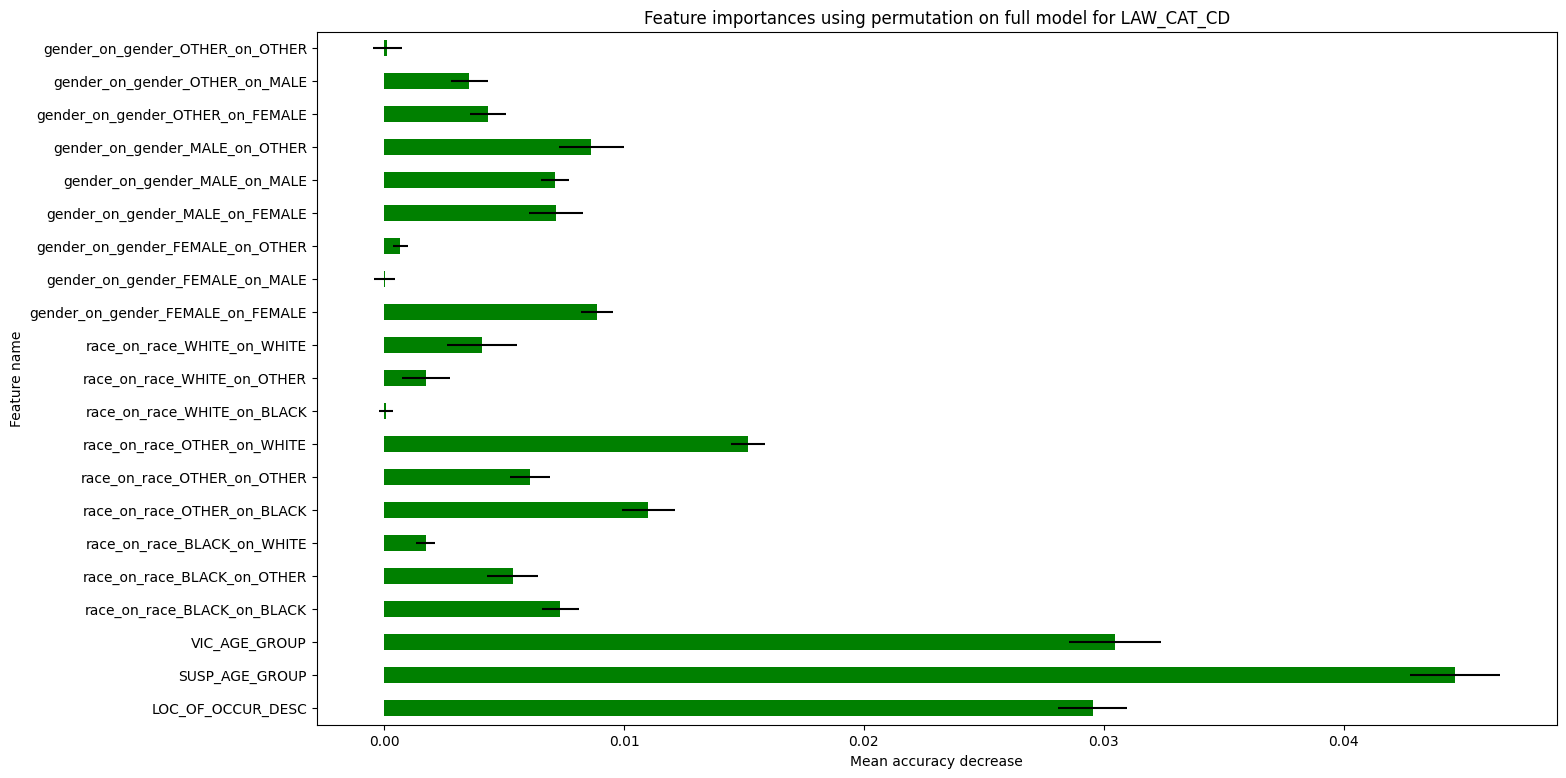
\includegraphics[width=\textwidth]{img/5.1.3/6/Feature importances using permutation on full model for LAW_CAT_CD.png}
                        \caption{Feature importances (permutation), w klasyfikacji law-breaking-level}
                        \label{goal_1_exp_6_imp_perm_law}
                    \end{figure}
                    
                    \begin{table}
                    \centering
                     \begin{tabular}{|c|c|c|c|}
                            \hline
                          Nazwa metryki & Wartość & Zmiana wartości & Klasyfikacja \\ \hline
                            Accuracy &  35,11\% & -0,215 & key-code\\ \hline
                            Accuracy &  54,465\% & +0,89 & law-breaking-level\\ \hline
                        \end{tabular}
                        \caption{Wyniki dla eksperymentu nr 6}
                        \label{goal_1_exp_6_results}
                     \end{table}
                     \FloatBarrier
                     Na podstawie spadków dokładności klasyfikacji dla obu cech, widocznych w tabelach \ref{goal_1_exp_4_results}, \ref{goal_1_exp_5_results} i \ref{goal_1_exp_6_results}, biorąc pod uwagę wpływ na wydajność rozwiązania, jaki ma tak duże rozwinięcie zbioru kolumn, pomysł przedstawiony w eksperymentach 4, 5 i 6 nie będzie dalej badany.
                }
                \paragraph{Eksperyment nr 7}{
                    W tym eksperymencie, postanowiono sprawdzić zachowanie klasyfikacji key-code przy dodaniu do zbioru cech, w oparciu o które jest dokonywana klasyfikacja kolumny law-breaking-level
                    \begin{figure}[!htbp]
                        \centering
                        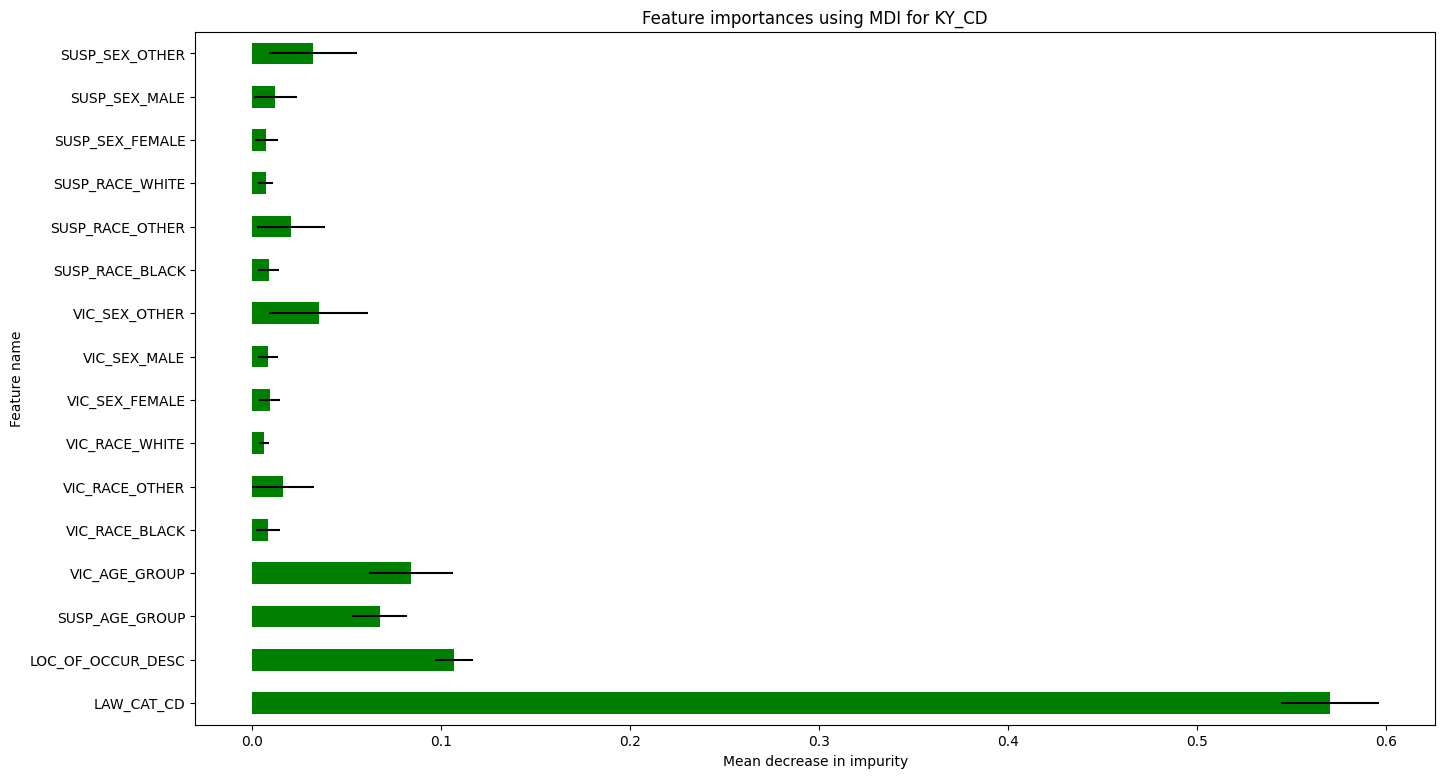
\includegraphics[width=0.9\textwidth]{img/5.1.3/7/Feature importances using MDI for KY_CD.png}
                        \caption{Feature importances (MDI), w klasyfikacji key-code}
                        \label{goal_1_exp_7_imp_mdi_key}
                    \end{figure}
                    
                    \begin{figure}[!htbp]
                        \centering
                        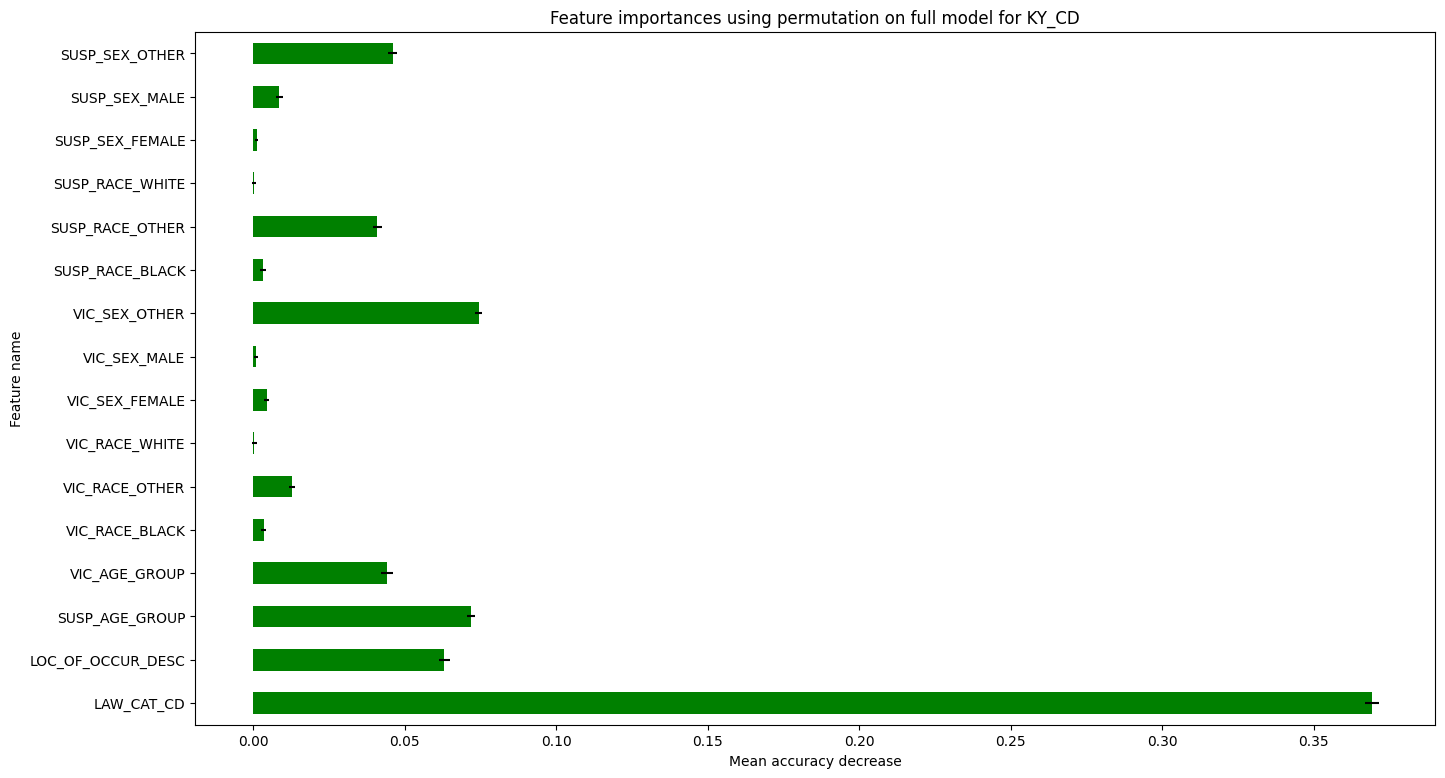
\includegraphics[width=0.9\textwidth]{img/5.1.3/7/Feature importances using permutation on full model for KY_CD.png}
                        \caption{Feature importances (permutation), w klasyfikacji key-code}
                        \label{goal_1_exp_7_imp_perm_key}
                    \end{figure}
                    
                    \begin{table}
                    \centering
                     \begin{tabular}{|c|c|c|c|}
                            \hline
                          Nazwa metryki & Wartość & Zmiana wartości & Klasyfikacja \\ \hline
                            Accuracy &  59,39\% & +24,28 & key-code\\ \hline
                        \end{tabular}
                        \caption{Wyniki dla eksperymentu nr 7}
                        \label{goal_1_exp_7_results}
                     \end{table}
                     \FloatBarrier
                     Na podstawie wzrostu dokładności klasyfikacji, widocznej w tabeli \ref{goal_1_exp_7_results} oraz wykresów \ref{goal_1_exp_7_imp_mdi_key} i \ref{goal_1_exp_7_imp_perm_key} pomysł aby dodać dodatkową cechę należy uznać za bardzo korzystny.
                }
                \paragraph{Eksperyment końcowy} {
                    W oparciu o przeprowadzone eksperymenty wyodrębniono zbiór cech, dla których klasyfikacja zostanie sprawdzona na całym zbiorze danych, wraz z doborem odpowiednich parametrów. Postanowiono skonfrontować to z wynikami na pełnym zbiorze, niepoddanym imputacji grup wiekowych. Jako parametry inne niż domyślnie dostarczane przez algorytm wybrano te uzyskane we wcześniejszej fazie projektu, tj. podczas eksperymentów z checkpointu nr 3, zostały one przedstawione w tabeli \ref{goal_1_exp_final_params}.
                    Wspomniany zbiór cech, wykorzystany w końcowej klasyfikacji składał się z: 
                    \begin{itemize}
                        \item LAW\_CAT\_CD - poziom popełnionego przestępstwa - tylko przy klasyfikacji key-code;
                        \item LOC\_OF\_OCCUR\_DESC - opis otoczenia zdarzenia;
                        \item SUSP\_AGE\_GROUP - Grupa wiekowa podejrzanego
                        \item SUSP\_RACE - Rasa podejrzanego
                        \item SUSP\_SEX - Płeć podejrzanego
                        \item VIC\_AGE\_GROUP - Grupa wiekowa ofiary
                        \item VIC\_RACE - Rasa ofiary
                        \item VIC\_SEX - Płeć ofiary
                    \end{itemize}
                    Sposób grupowania tych cech został opisany w odpowiedniej podsekcji, warto wspomnieć, że rasy zostały pogrupowane zgodnie ze zbiorem ["WHITE", "BLACK", "HISPANIC", "UNKNOWN", "OTHER"].
                    
                    \begin{table}
                    \small
                    \centering
                    \begin{tabular}{|c|c|}
                    \hline
                    Nazwa parametru & Wartość parametru \\ \hline
                        min\_samples\_leaf & 100\\ \hline
                        max\_depth & 15 \\ \hline
                        n\_estimators & 100 \\ \hline
                        max\_samples & 0.99  \\ \hline
                        \end{tabular}
                        \caption{Parametry klasyfikatora}
                        \label{goal_1_exp_final_params}
                     \end{table}

                     \begin{table}
                     \small
                     \centering
                     \begin{tabular}{|c|c|c|c|c|}
                            \hline
                            ID & Parametry domyślne & Accuracy & Imputacja grup wiekowych & Klasyfikacja \\ \hline
                            1 & Tak  &  52,254\% & Tak & key-code\\ \hline
                            2 & Tak &  58,33\% & Tak & law-breaking-level\\ \hline
                            3 & Tak  &  60,378\% & Nie & key-code\\ \hline
                            4 & Tak &  52,694\% & Nie & law-breaking-level\\ \hline
                            5 & Nie  &  52,071\% & Tak & key-code\\ \hline
                            6 & Nie &  58,312\% & Tak & law-breaking-level\\ \hline
                            7 & Nie  &  60,146\% & Nie & key-code\\ \hline
                            8 & Nie &  52,822\% & Nie & law-breaking-level\\ \hline
                        \end{tabular}
                        \caption{Wyniki klasyfikacji}
                        \label{goal_1_exp_final_results}
                     \end{table}  
                     
                     Dodatkowo dla scenariuszy z największą dokładnością klasyfikacji, spośród tych wykorzystujących niedomyślne parametry, tj. scenariusz nr 6 i 8, przygotowano macierze pomyłek, zamieszczone w tabelach \ref{goal_1_exp_final_results_matrix_1} i \ref{goal_1_exp_final_results_matrix_2}. Przygotowano je tylko dla klasyfikacji poziomu wykroczenia, ponieważ tutaj klasyfikowana jest mała liczba klas, dzięki czemu statystyka ta jest bardziej czytelna.
                     
                     \begin{table}
                     \small
                     \centering
                     \begin{tabular}{|c|c|c|}
                            \hline
                            VIOLATION & MISDEMEANOR & FELONY\\ \hline
                           36768 & 138446 &  16298\\ \hline
                           27891 & 718781  & 82192\\ \hline
                           11945 & 338206 & 104672 \\ \hline
                        \end{tabular}
                        \caption{Macierz pomyłek scenariusza 6 }
                        \label{goal_1_exp_final_results_matrix_1}
                     \end{table}
                     
                     \begin{table}
                     \small
                     \centering
                     \begin{tabular}{|c|c|c|}
                            \hline
                            VIOLATION & MISDEMEANOR & FELONY\\ \hline
                           23955 & 86421 &  3272\\ \hline
                           18145 & 221943  & 9316\\ \hline
                           7840 & 106419 & 13202 \\ \hline
                        \end{tabular}
                        \caption{Macierz pomyłek scenariusza 8 }
                        \label{goal_1_exp_final_results_matrix_2}
                     \end{table}
                     \FloatBarrier
                     
                }
            }
            
            \subsubsection{Dyskusja i wnioski} {
                Analizując wyniki końcowe przedstawione w tabeli \ref{goal_1_exp_final_results}, można zauważyć, że ustawienie parametrów klasyfikatora, wartościami wybranymi w checkpoincie nr 3, nie wpłynęło w sposób znaczący na wyniki, może to być spowodowane zbyt małym zbiorem testowym, na podstawie którego były ustalane wartości parametrów klasyfikatora. Warto zauważyć, że imputacja grup wiekowych poprzez przypisanie najczęściej występującej wartości, wpływa na wzrost dokładności klasyfikacji poziomu wykroczenia w sposób korzystny, natomiast wyniki klasyfikacji kodu przestępstwa, przy zastosowaniu tej metody jest niższy. Najwyższe wyniki dokładności jakie udało się uzyskać podczas klasyfikacji to kolejno dla klasyfikacji kodu przestępstwa i poziomu wykroczenia: ~60\% i ~58\%. Aby odpowiedzieć na pytanie czy to dużo, postanowiono zobrazować rozkład danych klasyfikowanych na dwóch wykresach.\\
                
                \begin{figure}[!htbp]
                    \centering
                    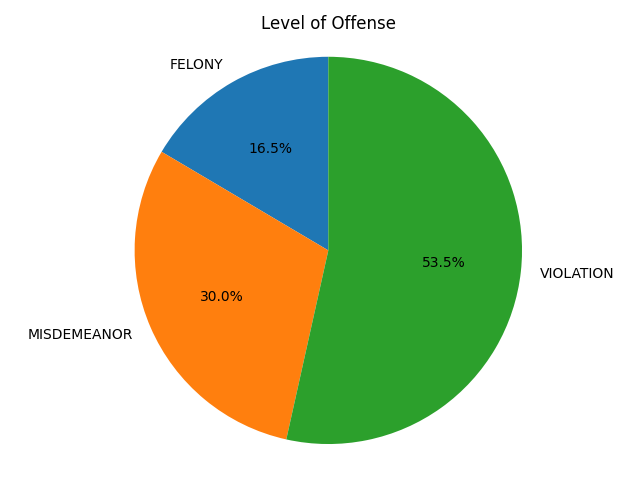
\includegraphics[width=\textwidth]{img/5.1.3/wnioski/offenseLevel.png}
                    \caption{Rozkład procentowy wartości poziomu wykroczenia.}
                    \label{goal_1_results_offenseLevel}
                \end{figure}
                
                \begin{figure}[!htbp]
                    \centering
                    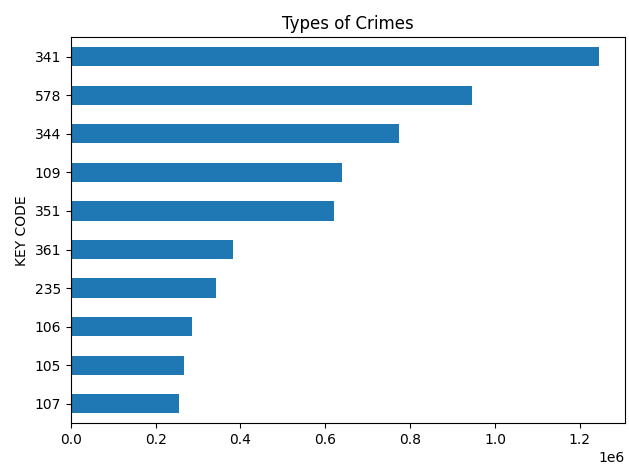
\includegraphics[width=\textwidth]{img/5.1.3/wnioski/typesOfCrimes.png}
                    \caption{Histogram 10 najczęstszych kodów przestępstwa.}
                    \label{goal_1_results_crimesTypes}
                \end{figure}
                \FloatBarrier
                                
                Na wykresie \ref{goal_1_results_offenseLevel} można zaobserwować, że najczęściej występującym zdarzeniem jest 'violation', które stanowi 53,5\% przypadków, klasyfikator osiągnął dokładność na poziomie ~58\%, można zatem stwierdzić, że nie klasyfikuje on w sposób losowy, a jego dokładność jest wyższa niż w przypadku, gdyby przyporządkowywał do każdego klasyfikowanego przypadku najczęściej występujący poziom.
                Z wykresu \ref{goal_1_results_crimesTypes} można wywnioskować, że kod 341 jest najczęściej występującym kodem przestępstwa, dodatkowe obliczenia pozwoliły wskazać, że występuje on w 16,87\% przypadków, na podstawie dokładności klasyfikacji na poziomie ~60\%, można uznać uzyskane wyniki klasyfikacji za bardzo dobre, gdyż nie zawężają się one do klasyfikacji tylko jednego kodu przestępstwa.
            }
        }
        \clearpage

        \subsection{Regresja godziny wystąpienia zdarzenia} \label{project_goal_2} {
        
            \subsubsection{Opis} {
                Regresja godziny wystąpienia zdarzenia jest zadaniem regresji i sprowadza się do przewidywania, w której sekundzie dnia wydarzyło się przestępstwo, na podstawie takich danych jak cechy podejrzanego i ofiary, otoczenia zdarzenia czy też pory roku i dnia tygodnia.

                Oryginalnie drugim celem była regresja czasu trwania przestępstwa, jednakże ze względu na bardzo nierównomierny rozkład (patrz charakterystyka zbioru) tej wartości, okazało się to zbyt trudne. Aby pozostać w temacie regresji oraz informacji na temat chwili wystąpienia zdarzenia, cel ten został przeformułowany do obecnej postaci. 

                Aby zrealizować ten cel wykorzystane zostaną algorytmy/modele przystosowane do zadania regresji. Głównie są to drzewa i lasy losowe zaimplementowane w popularnej bibliotece XGBoost. Wykonane zostało również wstępne przetwarzanie danych w oparciu o wcześniejszą analizę statystyczną. Wykorzystano takie metody jak redukcja wymiarów poprzez selekcję i ekstrakcję cech, oraz podstawowe techniki imputacji danych.
            }

            \subsubsection{Przygotowanie danych} {
                Wstępne przetwarzanie danych dla tego celu składa się z dwóch etapów. Pierwszy z nich dotyczy czyszczenia zbioru (m. in. imputacji) odrzucenia zbędnych danych, selekcji i ekstrakcji cech. Drugi dotyczy kodowania kolumn. Pierwszy etap można opisać w kontekście poszczególnych grup kolumn:
                \begin{enumerate}
                    \item Identyfikator
                    \begin{itemize}
                        \item Nie został wykorzystany - nie wnosi żadnej informacji
                    \end{itemize}
                    \item Typ zdarzenia
                    \begin{itemize}
                        \item Opisy słowne zostały odrzucone jako redundantne
                        \item Kod klasyfikacji wewnętrznej (PD\_CD) został odrzucony ze względu na zbyt dużą liczbę unikalnych wartości
                    \end{itemize}
                    \item Czy się udało
                    \begin{itemize}
                        \item Imputacja najczęstszą wartością (,,udało się'')
                    \end{itemize}
                    \item Data i czas zdarzenia
                    \begin{itemize}
                        \item Odrzucenie daty i czasu końca zdarzenia - dużo braków i nie wydaje się sensowne w kontekście estymacji godziny początku zdarzenia
                        \item Wyekstrahowanie dnia roku i dnia tygodnia oraz imputacja średnią
                        \item Wyekstrahowanie sekundy dnia i imputacja średnią
                    \end{itemize}
                    \item Data i czas zgłoszenia
                    \begin{itemize}
                        \item Odrzucone jako zbędne w kontekście tego celu
                    \end{itemize}
                    \item Otoczenie zdarzenia
                    \begin{itemize}
                        \item Wykorzystane obie kolumny
                        \item Brakujące dane nie są imputowane ze względu na znacząco liczne braki
                    \end{itemize}
                    \item Lokalizacja zdarzenia
                    \begin{itemize}
                        \item Odrzucona jako zbędna w kontekście tego celu
                    \end{itemize}
                    \item Cechy podejrzanego i ofiary
                    \begin{itemize}
                        \item Grupy wiekowe są ograniczone do wartości: <18, 18-24, 25-44, 45-64, 64+, NaN (nieznane)
                        \item Rasy UNKNOWN i OTHER są oznaczone jako NaN
                        \item Płcie są ograniczone do wartości: F (kobieta), M (mężczyzna), NaN (nieznane)
                    \end{itemize}
                \end{enumerate}
                Niezastosowanie imputacji i pozostawienie wartości NaN w niektórych kolumnach, jako ,,nieznane'' zostało wykonane ze względu na charakterystykę wykorzystanego algorytmu (XGBoost), który potrafi ,,radzić'' sobie z brakującymi wartościami. Zastosowanie prostej imputacji (np. wartość najczęstsza) w przypadku silnie wybrakowanych danych mogłoby znacząco obciążyć zbiór.
                
                Po drugim etapie wstępnego przetwarzania danych zbiór składa się z następujących kolumn, zakodowanych w następujący sposób:
                \begin{itemize}
                    \item CMPLNT\_DAY\_OF\_YEAR - wartość całkowita
                    \item CMPLNT\_DAY\_OF\_WEEK - wartość całkowita
                    \item KY\_CD - one hot encoding
                    \item LAW\_CAT\_CD - one hot encoding
                    \item CRM\_ATPT\_CPTD\_CD - one hot encoding (bez kolumny ,,ATTEMPTED'')
                    \item LOC\_OF\_OCCUR\_DESC - one hot encoding (bez kolumny NaN)
                    \item PREM\_TYP\_DESC - one hot encoding (bez kolumny NaN)
                    \item VIC\_SEX - one hot encoding (bez kolumny NaN)
                    \item SUSP\_SEX - one hot encoding (bez kolumny NaN)
                    \item VIC\_RACE - one hot encoding (bez kolumny NaN)
                    \item SUSP\_RACE - one hot encoding (bez kolumny NaN)
                    \item VIC\_AGE\_GROUP - ordinal encoding (wartości całkowite od 0 do 4)
                    \item SUSP\_AGE\_GROUP - ordinal encoding (wartości całkowite od 0 do 4)
                \end{itemize}
                
                Zbiór danych został podzielony na zbiory uczący (70\%) i testowy (30\%).
            }

            \subsubsection{Przetwarzanie i analiza danych} {
                Przetwarzanie i analiza danych została przeprowadzona z wykorzystaniem biblioteki XGBoost i algorytmów Gradient Boosted Tree oraz Gradient Boosted Random Forest. W celu optymalizacji hiperparametrów wykorzytano bibliotekę ,,optuna'', która przeszukuje określoną przestrzeń hiperparametrów z wykorzystaniem specjalizowanych algorytmów, w celu minimalizacji zadanej wartości.
                
                Przeprowadzonych zostało kilka eksperymentów, gdzie każdy jest pojedynczym uruchomieniem algorytmu ,,optuna'' w celu znalezienia optymalnych wartości hiperparametrów dla modelu Gradient Boosted Tree (Forest) z biblioteki XGBoost. Przeszukiwane zakresy hiperparametrów za każdym razem są następujące:
                \begin{itemize}
                    \item eta - [0.1 - 1]
                    \item max\_depth - [3, 10]
                    \item min\_child\_weight - [1, 10]
                    \item subsample - [0.6, 1]
                    \item colsample\_bynode - [0.6, 1]
                    \item num\_parallel\_tree - [1, 10]
                \end{itemize}
                Pozostałe hiperparametry trenigu są następujące:
                \begin{itemize}
                    \item tree\_method - gpu\_hist
                    \item objective - reg:squarederror
                    \item eval\_metric - RMSE, MAE
                    \item num\_boost\_rounds - 100
                    \item early\_stopping\_rounds - 10
                \end{itemize}
                Optymalizowaną metryką przez bibliotekę ,,optuna'' jest MAE na zbiorze testowym (pełniącego w tym przypadku rolę zbioru walidacyjnego).
                
                Eksperymenty różnią się między sobą jedynie odrzuceniem niektórych ze zdefiniowanego w poprzedniej sekcji zbioru kolumn.
                
                \paragraph{Eksperyment 1.} W tym przypadku wykorzystane zostały wszystkie dostępne kolumny. Znalezione optymalne wartości parametrów:
                \begin{itemize}
                    \item eta - 0.79
                    \item max\_depth - 10
                    \item min\_child\_weight - 4.87
                    \item subsample - 0.9
                    \item colsample\_bynode - 0.85
                    \item num\_parallel\_tree - 9
                \end{itemize}
                Wartości metryk:
                \begin{itemize}
                    \item RMSE (zbiór uczący) - 22831
                    \item MAE (zbiór uczący) - 18647
                    \item RMSE (zbiór testowy) - 23120
                    \item MAE (zbiór testowy) - 18887
                \end{itemize}
                \begin{figure}[!htbp]
                    \centering
                    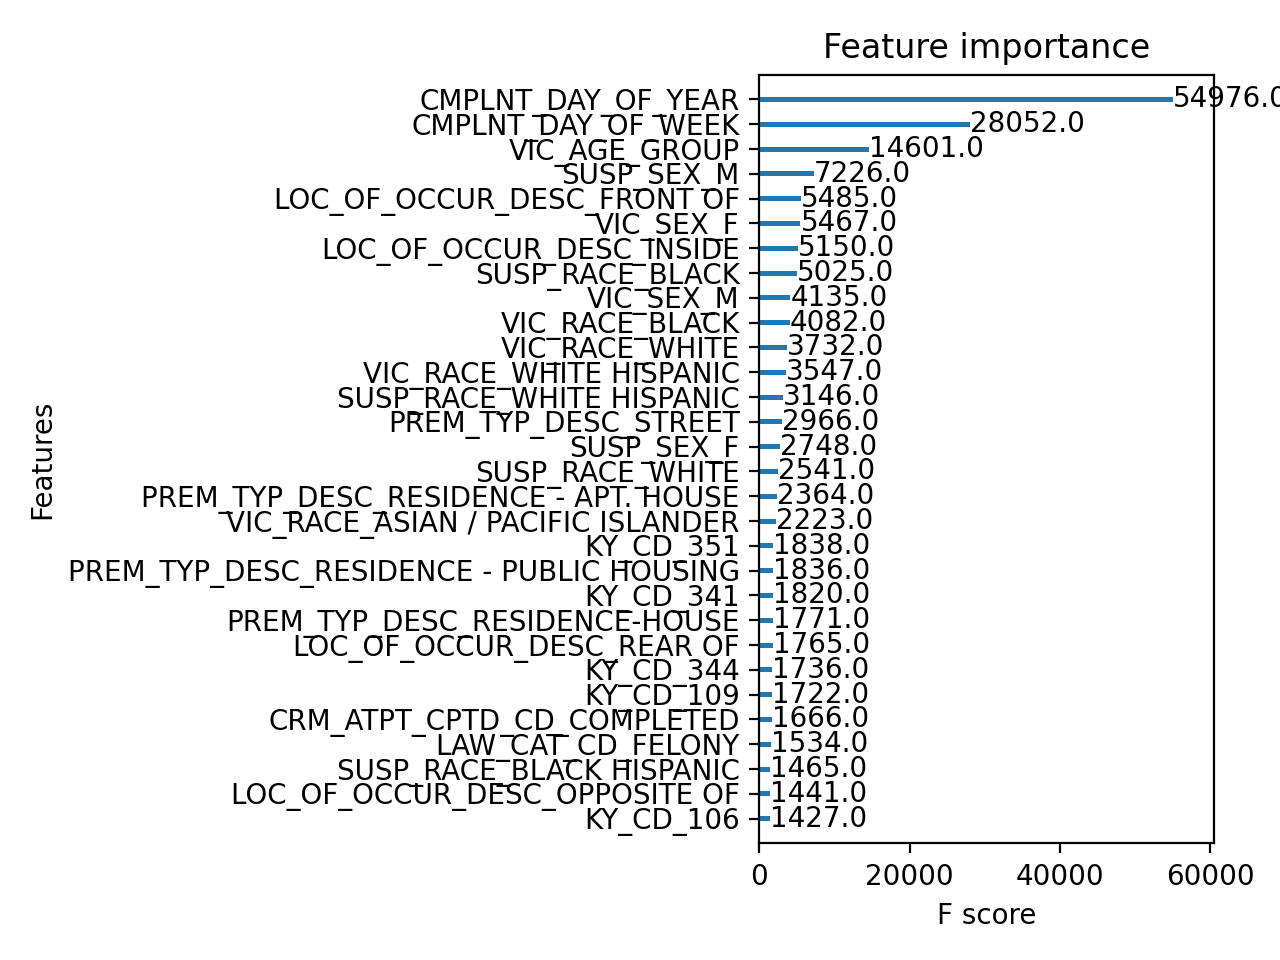
\includegraphics[width=\textwidth]{img/importance_1.png}
                    \caption{Wykres znaczenia poszczególnych cech dla modelu wyuczonego w eksperymencie 1.}
                    \label{importance_1}
                \end{figure}
                \FloatBarrier
                
                \paragraph{Eksperyment 2.} W tym eksperymencie nie wykorzystano informacji na temat typu zdarzenia. Znalezione optymalne wartości parametrów:
                \begin{itemize}
                    \item eta - 0.57
                    \item max\_depth - 10
                    \item min\_child\_weight - 3.47
                    \item subsample - 0.83
                    \item colsample\_bynode - 0.88
                    \item num\_parallel\_tree - 9
                \end{itemize}
                Wartości metryk:
                \begin{itemize}
                    \item RMSE (zbiór uczący) - 23118
                    \item MAE (zbiór uczący) - 18993
                    \item RMSE (zbiór testowy) - 23450
                    \item MAE (zbiór testowy) - 19282
                \end{itemize}
                \begin{figure}[!htbp]
                    \centering
                    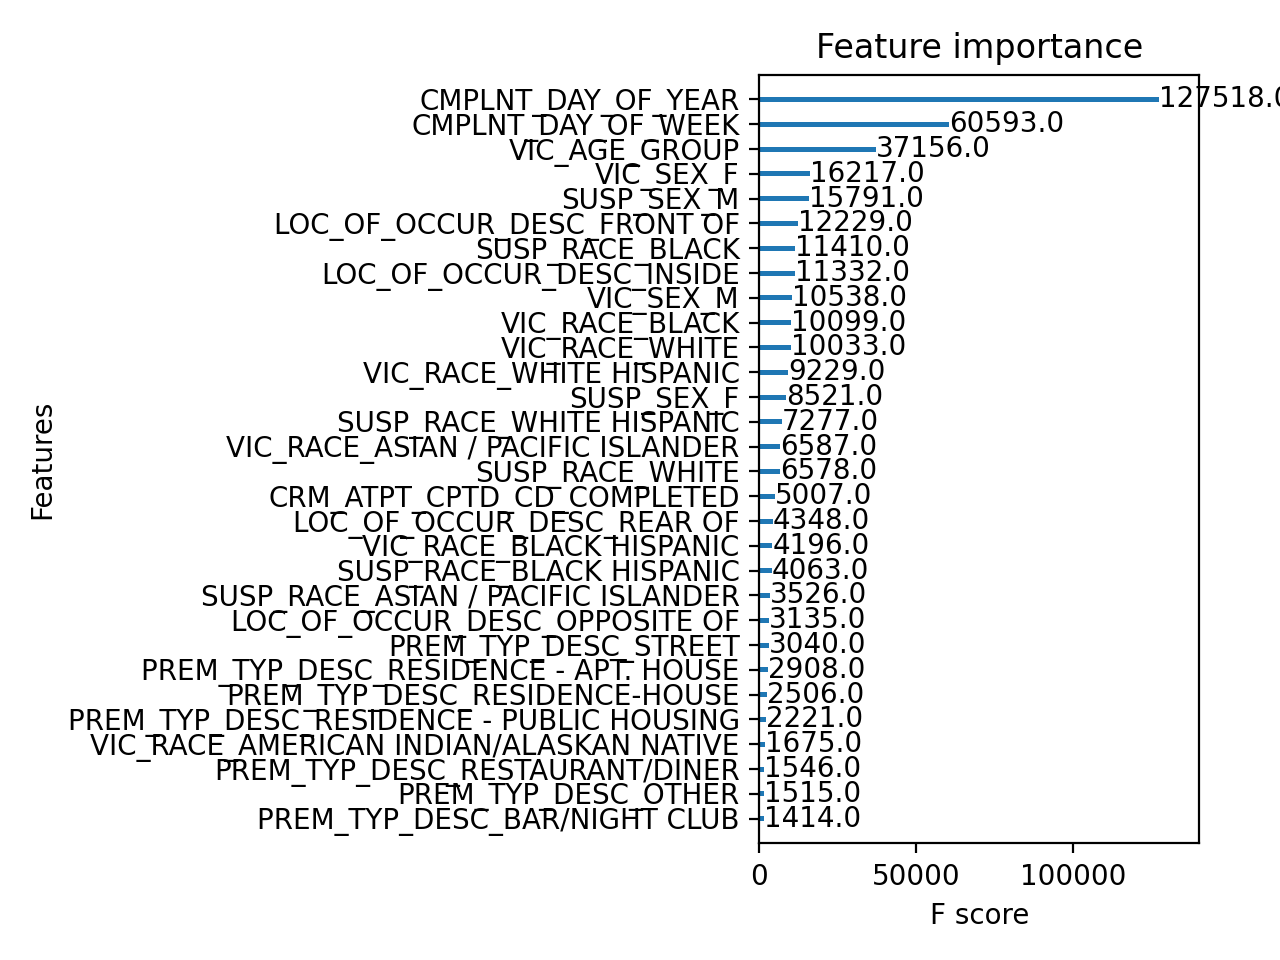
\includegraphics[width=\textwidth]{img/importance_2.png}
                    \caption{Wykres znaczenia poszczególnych cech dla modelu wyuczonego w eksperymencie 2.}
                    \label{importance_2}
                \end{figure}
                \FloatBarrier
            }

            \subsubsection{Dyskusja i wnioski} {
                W eksperymencie 1. wykorzystane zostały wszystkie dostępne dane, które wydają się przydatne dla tego zadani, zakodowane w optymalny sposób tak, aby nie stracić żadnej informacji. Podsumowując dostępne cechy można opisać realizowane zadanie, jako regresja godziny zdarzenia na podstawie cech jego typu, cech jego uczestników, otoczenia i pory roku oraz dnia tygodnia.
                
                Po przeprowadzeniu wszystkich niezbędnych obliczeń znalezione zostały optymalne hiperparametry, dla których model osiągnął wartość średniego błędu bezwzględnego równą 18887 sekund, na zbiorze testowym oraz 18647 sekund na zbiorze uczącym. Pierwszym spostrzeżeniem jest, że wartości te bardzo są do siebie zbliżone (obie wynoszą trochę ponad 5 godzin), co oznacza, że model ma niską wariancję i nie został przetrenowany. Z drugiej strony oznacza to, że najprawdopodobniej można osiągnąć jeszcze trochę lepsze wyniki, zbliżając się do momentu, w którym dojdzie do przetrenowania. Być może potrzebny jest dłuższy trening. Obserwując nieprzedstawione tu metryki podczas uczenia widać jednak, że wartości te zmieniają się po 100 rundach już bardzo nieznacznie.
                
                Jeżeli chodzi o interpretację wartości średniego błędu bezwzględnego, to oznacza on, że średnio udaje się przewidzieć godzinę zdarzenia z dokładnością do około 5 godzin. Innymi słowy, można ocenić porę dnia - czy jest ranek, popołudnie, wieczór czy noc. Wydaje się, że informacja ta może być jak najbardziej przydatna. Z jednej strony trzeba jednak przyznać, że nie jest to bardzo spektakularny wynik i gdyby udało się estymować z dokładnością do godziny byłoby to znacznie ciekawsze osiągnięcie. Z drugiej strony natomiast, osiągnięcie tak dużej dokładności przy takim zbiorze dostępnych cech może okazać się zupełnie niemożliwe.
                
                Rysunek \ref{importance_1} pokazuje znaczenie poszczególnych cech dla wyuczonego modelu. Widać tutaj, że najbardziej istotna jest pora roku i pora tygodnia, oraz cechy podejrzanego i ofiary. Zwłaszcza pora roku wydaje się być logiczna, ponieważ zależnie od pory roku o danej porze dnia jest już ciemno lub jeszcze nie. Duże znaczenie ma też czy zdarzenie miało miejsce na zewnątrz czy wewnątrz np. budynku.
                
                Drugi przeprowadzony eksperyment daje bardzo nieznacznie gorsze wyniki. Tym razem dla zbioru testowego MAE 19282 sekund a dla zbioru uczącego 18993. Ponownie nie mamy tu do czynienia z przetrenowaniem i ponownie jakość regresji praktycznie przestała się poprawiać. Okazuje się więc, że rezygnacja z nawet mniej znaczących kolumn pogarsza jakość regresji i sytuacja taka miałaby miejsce prawdopodobnie dla dowolnych innych cech. Wynika to z faktu, że wyuczony model znajduje bardzo złożone i subtelne zależności, tak więc praktycznie każda cecha może okazać się przydatna. Dodatkowo należy zwrócić uwagę, że algorytmy lasu losowego nie są tak bardzo podatne na obecność nadmiarowych i nieprzydatnych kolumn. Na rysunku \ref{importance_2} te same cechy okazują się być istotne, jak w przypadku pierwszego eksperymentu.
                
                \paragraph{Wnioski} z przeprowadzonych badań są następujące:
                \begin{itemize}
                    \item Dla wielu kombinacji hiperparametrów model osiąga bardzo podobne wyniki
                    \item Osiągnięta dokładność zawsze znajduje się w okolicach 5 godzin co pozwala ocenić porę dnia zdarzenia
                    \item Najistotniejszymi cechami okazują się pora roku i dzień tygodnia
                    \item Rezygnacja z danych o typie zdarzenia powoduje obniżenie jakości regresji
                \end{itemize}
            }
        }
        \newpage

        \subsection{Grupowanie przestępstw na podstawie podzbiorów cech}
        \label{project_goal_3} {
            \subsubsection{Opis} {
                Oryginalnie spośród cech podejrzanego i ofiary miał zostać wybrany kilkakrotnie  podzbiorów podzbiór cech, które utworzą
                przedmiot eksperymentu - etykietę, a dla każdej z 
                nich (która może być złożeniem kilku atrybutów) miała być przeprowadzona
                seria eksperymentów, mająca na celu automatyczne pogrupowanie zdarzeń
                zgodnie z tą etykietą, wykorzystując wszystkie pozostałe atrybuty (poza
                tworzącymi etykietę). Koncept ten został porzucony ze względu na wysoką złożoność obliczeniową przy wyborze permutacji najlepszego zestawu przetworzonych danych.
                
                W ramach tego celu zostało przeprowadzone grupowanie zdarzeń na podstawie etykiety związanej z poziomem przestępstwa. Zostały do tego wykorzystane cechy osoby podejrzanej, poszkodowanej oraz informacje o czasie wystąpienia danego zdarzenia.
                
                Po przeprowadzeniu grupowania z wykorzystaniem kilku
                różnych algorytmów (kmeans oraz kmodes), zmierzona
                została jakość grupowania za pomocą metryk, a same dane zwizualizowano, aby ocenić jakość klasteryzacji.
                
                \begin{figure}[!htbp]
                    \centering
                    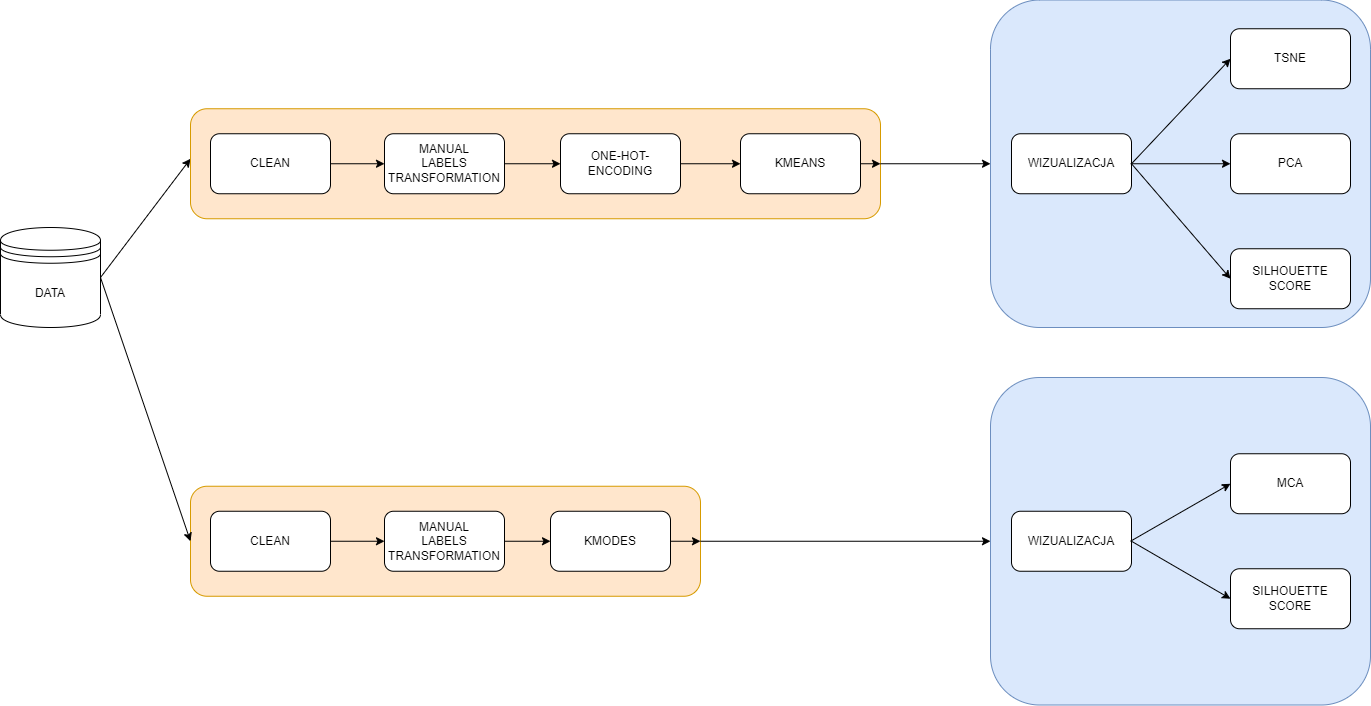
\includegraphics[width=1\textwidth]{img/clustering/Scheme.png}
                    \caption{Schemat realizacji celu - pipeline}
                    \label{scheme}
                \end{figure}
                \FloatBarrier
            }

            \subsubsection{Przygotowanie danych} {
                Przez rozpoczęciem eksperymentów z pełnego zestawu kolumn zostały wybrane te opisujące zarówno podejrzanego, jak i ofiarę, które składały się z informacji o płci, grupie wiekowej, oraz rasie. Informacje o grupie wiekowej zostały zmodyfikowane, aby reprezentowały dane z przedziału 0 do 1.
                
                \begin{table}[!htbp]
                    \small
                    \centering
                    \begin{tabular}{|c|c|}
                        \hline
                        Początkowa wartość grupy wiekowej & Wartość po transformacji \\ \hline
                        <18 & 0 \\
                        18-24 & 0.25 \\
                         25-44 & 0.5 \\
                        45-64 & 0.75 \\ 
                        65+ & 1 \\ \hline
                    \end{tabular}
                    \caption{Wartości kolumny zawierającej dane o grupie wiekowej po przekształceniu}
                    \label{trans_age}
                \end{table}
                \FloatBarrier
                
                Ponadto, w analizie brana była pod uwagę pora dnia zdarzenia, która została wyekstrahowana z godziny zgłoszenia, a następnie zamieniona na dane kategoryczne.
                
                \begin{table}[!htbp]
                    \small
                    \centering
                    \begin{tabular}{|c|c|}
                        \hline
                        Początkowa wartość godziny & Wartość po transformacji \\ \hline
                        od 1 do 5 & BEFORE\_DAWN \\
                        5 do 12 & MORNING \\
                         12 do 17 & AFTERNOON \\
                        17 do 20 & EVENING\\
                        20 do 23 & NIGHT\\ 
                        0 & MIDNIGHT \\ \hline
                    \end{tabular}
                    \caption{Wartości kolumny zawierającej dane o wystąpieniu zdarzenia po przekształceniu}
                    \label{trans_occurance}
                \end{table}
                \FloatBarrier
                
                W celu przeprowadzenia eksperymentów wzięte pod uwagę rekordy, nie mogły posiadać wybrakowanych danych w ramach opisanych kolumn. Dodatkowo, brane pod uwagę były wyłącznie rekordu w których wartość płci oznaczała kobietę, lub mężczyznę. Pozwoliło to na wyszczególnienie \textbf{2301826} rekordów, które zostały poddane analizie. Usunięta została również kolumna zawierając kod przestępstwa, gdyż stanowiła ona etykiety do późniejszej weryfikacji. 
            }

            \subsubsection{Przetwarzanie i analiza danych} {
                Każdy z algorytmów wymagał dodatkowego przetworzenia rekordów, które będą stanowiły dane eksperymentu. W przypadku algorytmu KMeans dane kategorialne zostały poddane operacji one hot encodingu, aby poprawnie przeprowadzić klasteryzację. Liczba klastrów została ustawiona zgodnie z liczbą etykiet poziomów przestępstw na 3.
                
                Po uzyskanych wynikach klasteryzacji rozpatrywany był każdy przepadek dopasowania danej etykiety do klastra, a następnie wybrany został wariant z największą wartością accuracy.
                
                \begin{table}[!htbp]
                \centering
                \begin{tabular}{|c|c|c|c|}
                    \hline
                    LABEL 0 & LABEL 1 & LABEL 2 & Accuracy \\ \hline
                    FELONY  & VIOLATION  & MISDEMEANOR & 36.837 \\
                    \hline
                \end{tabular}
                \caption{Najlepsza permutacja dla eksperymentu KMeans}
                \label{tab:kmeans_lab}
                \end{table}
                
                \begin{table}[!htbp]
                \centering
                \begin{tabular}{|c|c|c|c|}
                    \hline
                    & FELONY  & VIOLATION  & MISDEMEANOR \\ \hline
                    DATASET & 562577 & 714884 & 1024365 \\
                    CLUSTER & 863971 & 697736 & 740119 \\ 
                    \hline
                \end{tabular}
                \caption{Liczebność próbek danych etykiet dla zbioru danych i klastrów}
                \label{tab:kmeans_samples}
                \end{table}
                
                \begin{table}[!htbp]
                \centering
                \begin{tabular}{|c|c|c|c|c|}
                    \hline
                 & VIOLATION  &  MISDEMEANOR & FELONY\\ \hline
                accuracy            &  0.597510  &   0.524523 &  0.614722  \\
                precision      &        0.348382  &   0.452642 & 0.312340 \\
                recall        &        0.340026   &  0.327041 & 0.479673   \\
                sensitivity     &       0.340026  &   0.327041 & 0.479673   \\
                specificity     &      0.713501   &  0.682879 & 0.658405  \\
                    \hline
                \end{tabular}
                \caption{Wartości poszczególnych metryk dla uzyskanych klastrów - KMeans}
                \label{tab:kmeans_metrics}
                \end{table}
                
                W celu wizualizacji otrzymanych klastrów w wyniku algorytmu KMeans została zastosowana metoda redukcji wymiarów PCA (\textit{Principal component analysis}), której wynikiem były dane dwuwymiarowe. 
                
                
                \begin{figure}[!htbp]
                    \centering
                    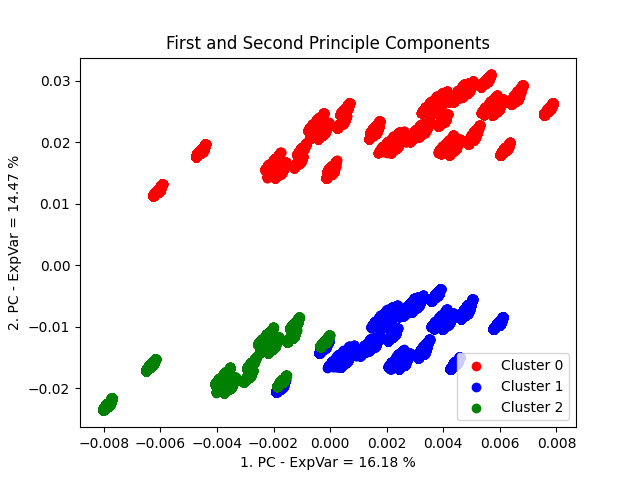
\includegraphics[width=0.9\textwidth]{img/clustering/pca_plot.png}
                    \caption{Wykres przedstawiający wyniki klasteryzacji po zastosowaniu PCA}
                    \label{clust_pca}
                \end{figure}
                \FloatBarrier
                
                \begin{figure}[!htbp]
                    \centering
                    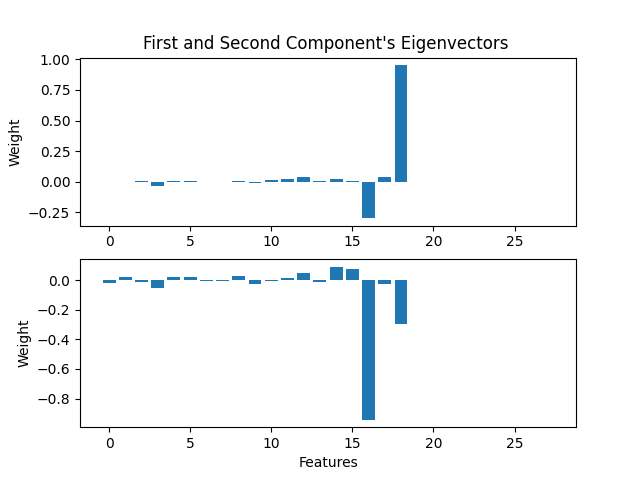
\includegraphics[width=0.9\textwidth]{img/clustering/pca_weights.png}
                    \caption{Wagi cech wektorów własnych PCA}
                    \label{clust_pca_weights}
                \end{figure}
                \FloatBarrier
                
                Ponadto została wyznaczona średnia wartość silhouette score, które w przypadku eksperymentu KMeans wynosiła \textbf{0.61}
                
                 \begin{figure}[!htbp]
                    \centering
                    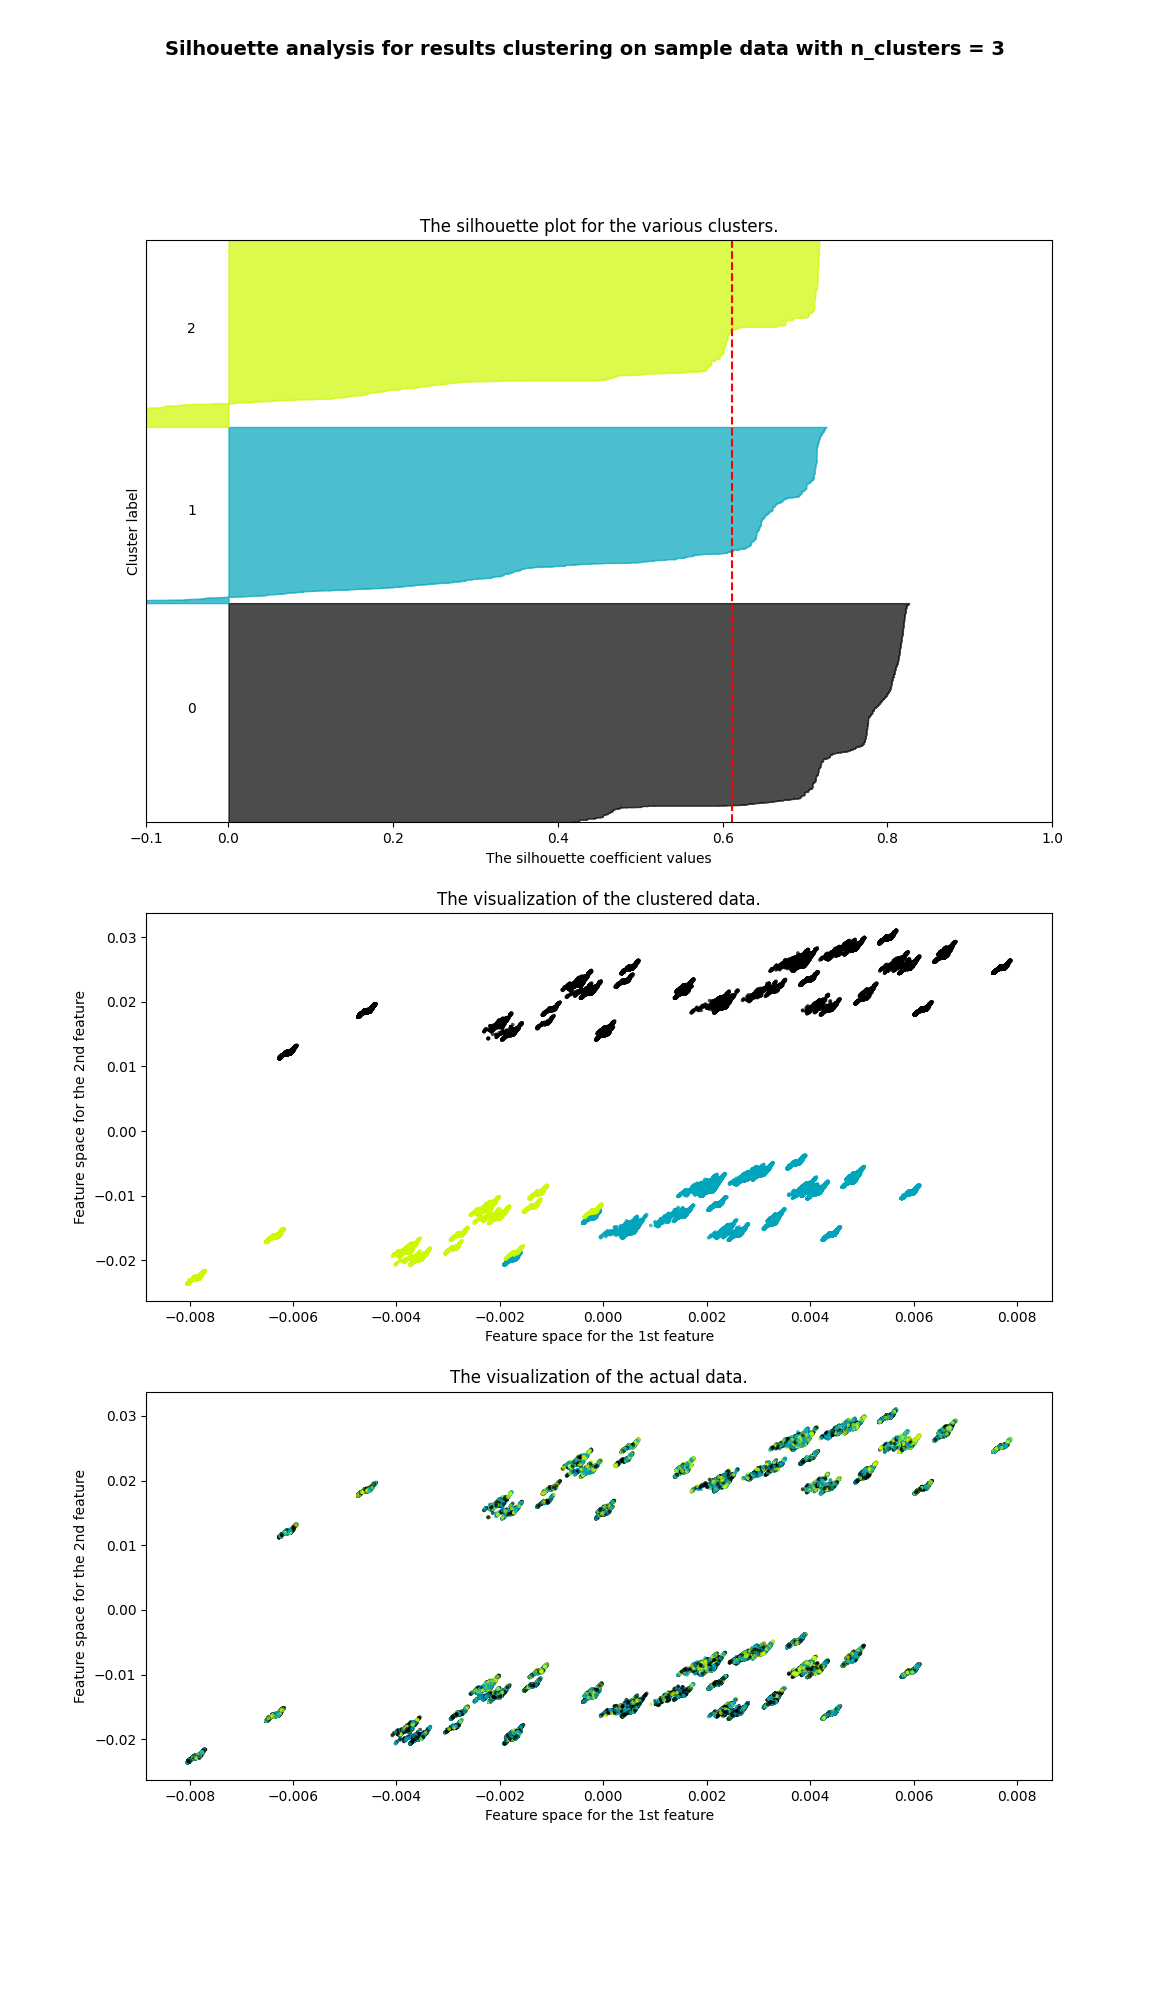
\includegraphics[width=1\textwidth]{img/clustering/kmeans_silh_crime_codes.png}
                    \caption{Silhouette score poszczególnych próbek oraz porównanie wizualne danych z etykietą po klastrowaniu oraz faktyczną dla algorytmu KMeans}
                    \label{silh_kmeans}
                \end{figure}
                \FloatBarrier
                
                 \begin{figure}[!htbp]
                    \centering
                    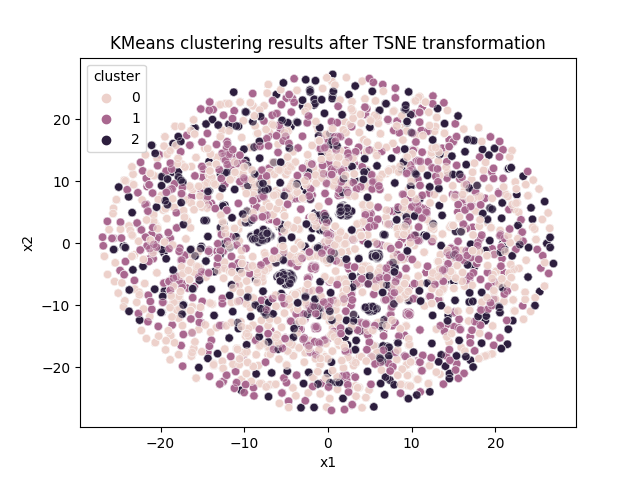
\includegraphics[width=0.85\textwidth]{img/clustering/tsne_crime_codes_clusters.png}
                    \caption{Wizualizacja danych przetworzonych za pomocą algorytmu TSNE - dane po klasteryzacji}
                    \label{tsne_clusters}
                \end{figure}
                \FloatBarrier
                
                \begin{figure}[!htbp]
                    \centering
                    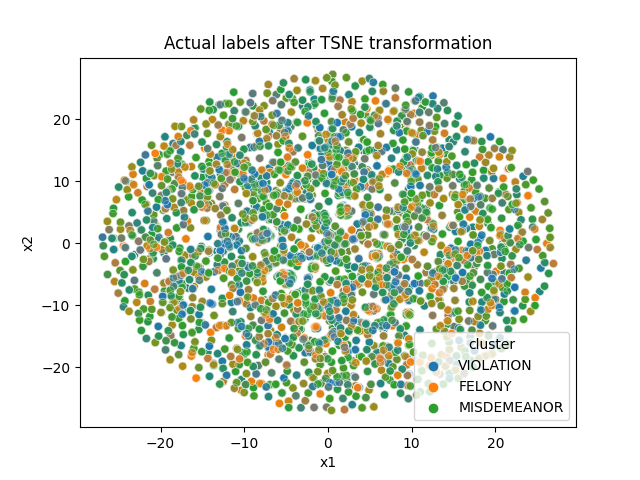
\includegraphics[width=0.85\textwidth]{img/clustering/tsne_crime_codes_actual.png}
                    \caption{Wizualizacja danych przetworzonych za pomocą algorytmu TSNE - dane faktyczne}
                    \label{tsne_actual}
                \end{figure}
                \FloatBarrier
                
                \textbf{Drugi eksperyment} przeprowadzono z wykorzystaniem algorytmu KModes, który jest silnie nastawiony na wykorzystanie danych kategorialnych i wydawał się w przypadku analizowanego zbioru obiecującym wyborem.
                
                Ponieważ algorytm ten bazuje na danych kategorialnych kolumny nie musiały zostać poddane one-hot encodingowi.
                
                \begin{table}[!htbp]
                \centering
                \begin{tabular}{|c|c|c|c|}
                    \hline
                    LABEL 0 & LABEL 1 & LABEL 2 & Accuracy \\ \hline
                    MISDEMEANOR  & VIOLATION  & FELONY  & 52.32 \\
                    \hline
                \end{tabular}
                \caption{Najlepsza permutacja dla eksperymentu KModes}
                \label{tab:kmodes_lab}
                \end{table}
                
                \begin{table}[!htbp]
                \centering
                \begin{tabular}{|c|c|c|c|}
                    \hline
                    & FELONY  & VIOLATION  & MISDEMEANOR \\ \hline
                    DATASET & 562577 & 714884 & 1024365 \\
                    CLUSTER & 211447 & 504967 & 1585412 \\ 
                    \hline
                \end{tabular}
                \caption{Liczebność próbek danych etykiet dla zbioru danych i klastrów}
                \label{tab:kmodes_samples}
                \end{table}
                
                \begin{table}[!htbp]
                \centering
                \begin{tabular}{|c|c|c|c|c|}
                    \hline
                 & VIOLATION  &  MISDEMEANOR & FELONY \\ \hline
                accuracy      &  0.689722     & 0.610955 & 0.745811      \\
                precision   &        0.500672  &   0.540637 & 0.446746 \\
                recall       &       0.353656  &   0.836745 & 0.167911 \\
                sensitivity    &       0.353656  &   0.836745 & 0.167911   \\
                specificity   &      0.841113  &   0.429900 & 0.932739 \\
                    \hline
                \end{tabular}
                \caption{Wartości poszczególnych metryk dla uzyskanych klastrów - KModes}
                \label{tab:kmodes_metrics}
                \end{table}
                
                Również w tym przypadku wizualizacja danych wymagała redukcji wymiarowości. Zamiana danych na zgodne z PCA jest błędne, dlatego zastosowana została metoda MCA (ang. \textit{Multiple correspondence analysis}) przystosowana do danych kategorialnych.
                
                 \begin{figure}[!htbp]
                    \centering
                    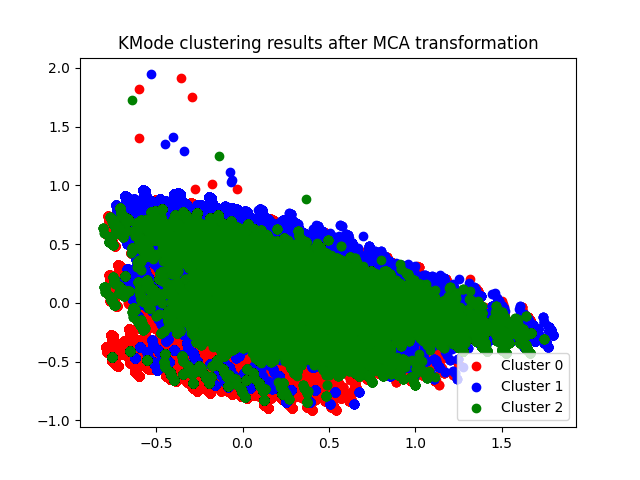
\includegraphics[width=0.85\textwidth]{img/clustering/mca.png}
                    \caption{Wykres przedstawiający wyniki klasteryzacji po zastosowaniu MCA}
                    \label{clust_mca}
                \end{figure}
                \FloatBarrier
                
               Dla eksperymentu z algorytmem KModes również wyznaczono wartość silhouette score, które wynosiła \textbf{0.07}.
                
                 \begin{figure}[!htbp]
                    \centering
                    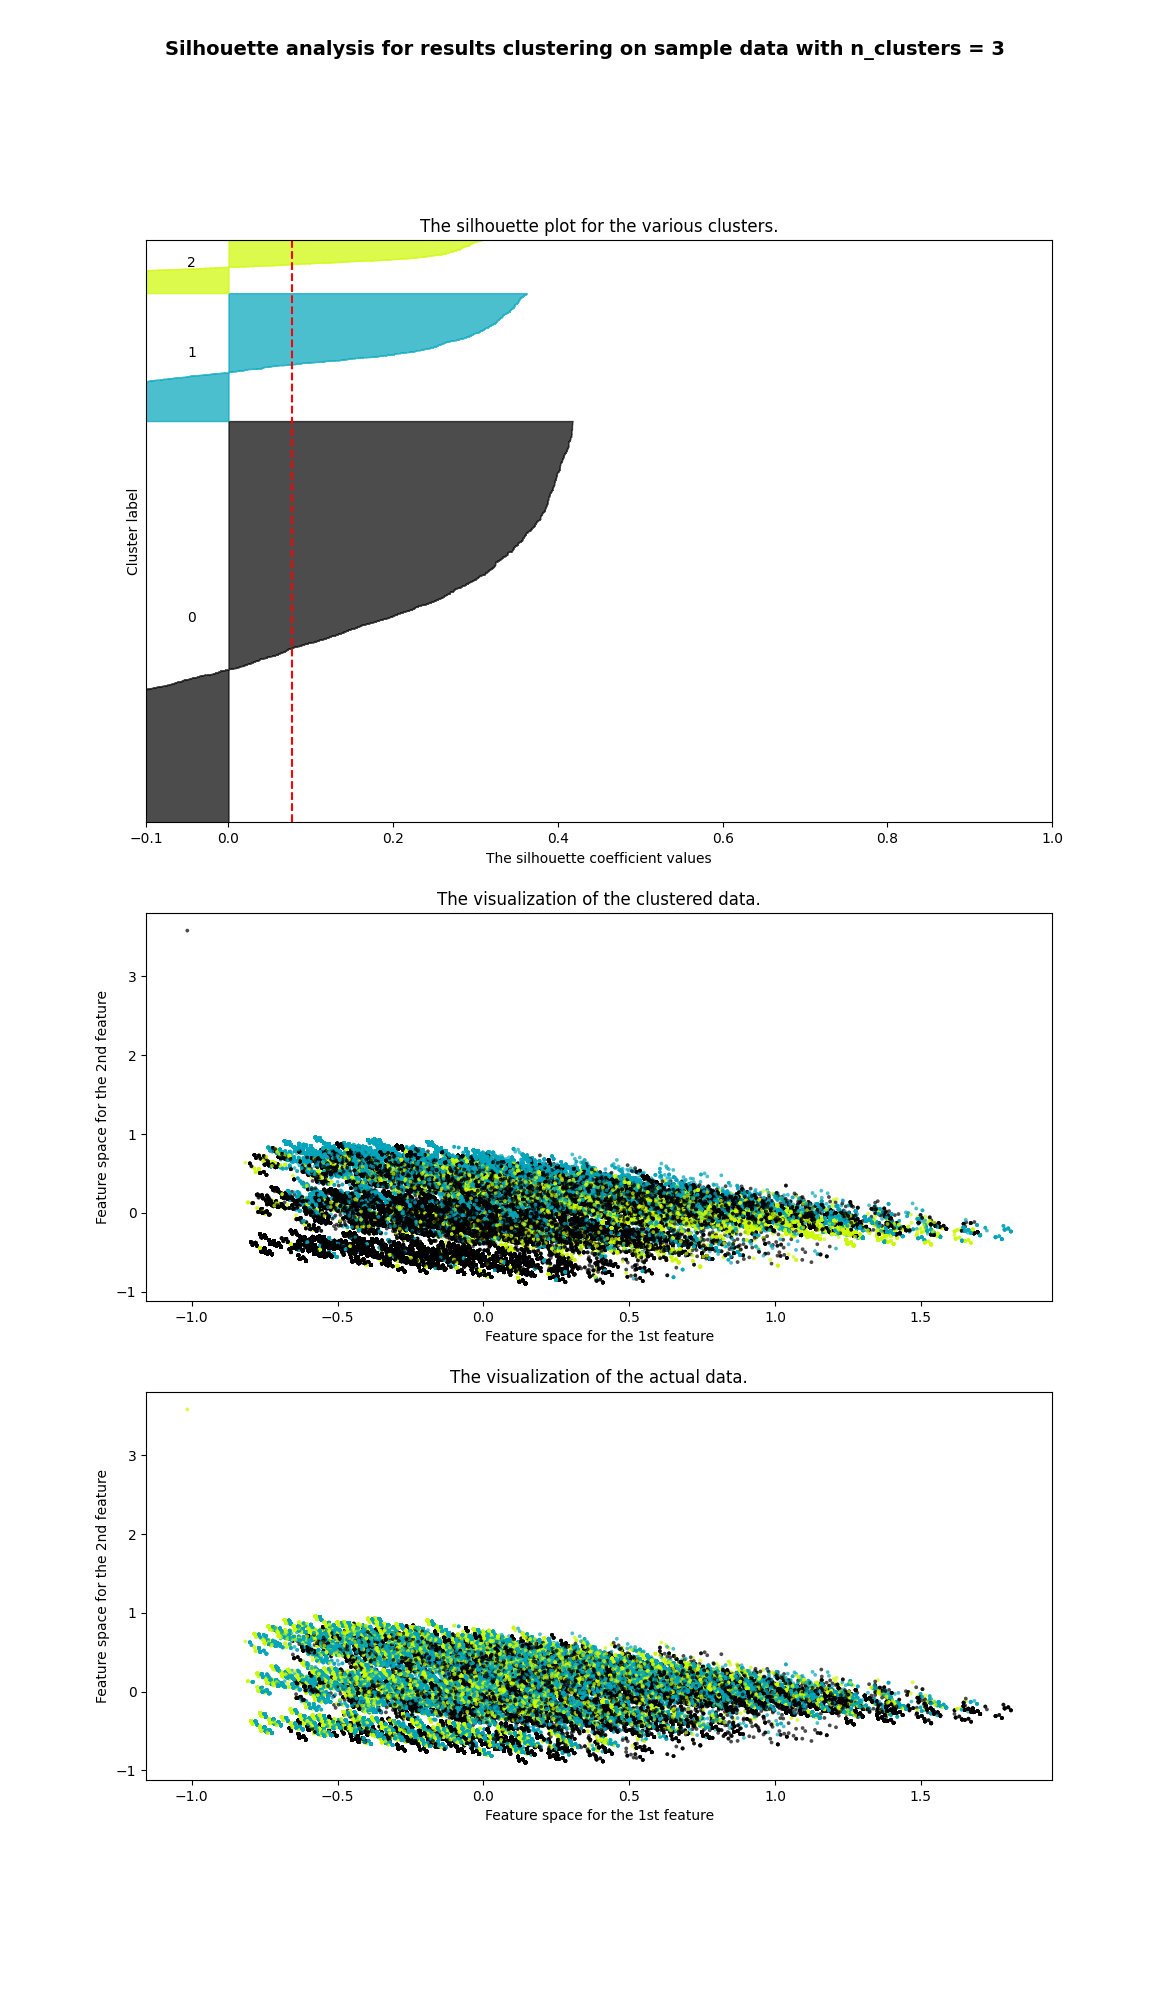
\includegraphics[width=1\textwidth]{img/clustering/kmodes_silhouette.png}
                    \caption{Silhouette score poszczególnych próbek oraz porównanie wizualne danych z etykietą po klastrowaniu oraz faktyczną dla algorytmu Kmodes}
                    \label{silh_kmodes}
                \end{figure}
                \FloatBarrier
            }

            \subsubsection{Dyskusja i wnioski} {
                 W przypadku algorytmu KMeans można zauważyć w tabeli \ref{tab:kmeans_metrics} niższą wartość accuracy dla algorytmu KModes. Przeprowadzenie redukcji wymiarów za pomocą metody PCA zwróciło wartość wariancji oscylującą około 15\%, co jest dalekie od optymalnych wartości referencyjnych 70\% - 80\%. Rozkład liczby próbek uzyskanej przez klastrowanie nie odpowiada wartościom występującym w faktycznym zbiorze danych. Ponadto, w przypadku każdej z etykiet miary precision oraz recall nie przekroczyły 50\% próbek, a większość oscylowała wokół 35\%.
                 
                 Algorytm KModes poradził sobie lepiej w przypadku rozważanego problemu. Accuracy otrzymane dla tego eksperymentu przekroczyło 50\%. Wyniki MCA pozwalają też na zaobserwowanie ułożenia danych, które są bardziej skupione i łatwiejsze do klasteryzacji. Metoda utworzyła klastry, z których jeden zawsze był znacznie większy. Przy założeniu, że ten klaster otrzymałby etykietę najliczniejszej grupy danych (MISDEMEANOR) przełożyłoby się to na wysokie wartości metryk precision oraz recall kosztem jakości klasteryzacji dla najmniejszego klastra (w tym przypadku FELONY).
                 
                 \textbf{Wnioski}:
                 \begin{itemize}
                     \item Zastosowanie algorytmu KMeans bez odpowiedniego przygotowania danych za pomocą one-hot encodingu prowadzi do uzyskania losowych wyników (najczęściej accuracy 1/n)
                     \item Algorytm KMeans nie pozwala na uzyskanie stabilnych wyników w przypadku danych kategorialnych
                     \item Algorytm KModes oferuje lepsze wyniki dla danych kategorialnych
                 \end{itemize}
            }
        }
        \newpage
    }
    
    \section{Ewolucja projektu} {
        Od momentu kiedy rozpoczęte zostały prace nad tym projektem nastąpiło bardzo wiele zmian dotyczących zarówno realizowanych celów, sposobów ich realizacji jak również zmian związanych ze świadomością i wiedzą uczestników projektu.
        
        Pierwszym znaczącym błędem, który został popełniony, było niedokładne przeanalizowanie danych pod kątem statystycznym. Należało dokładnie zbadać jaki jest rozkład wartości we wszystkich kolumnach i gdzie to tylko możliwe dokonać wizualizacji, które zawsze pomagają zrozumieć dane ludzkiemu odbiorcy. W ten sposób znacznie łatwiej byłoby sformułować sensowne cele. Ponieważ zabrakło tej analizy od samego początku, dwa cele zostały sformułowane nie do końca rozsądnie i uległy modyfikacjom.
        
        Drugim ważnym krokiem, który został podjęty w trakcie realizacji projektu a nie został zrealizowany wcześniej było skupienie się na temacie wstępnego przetwarzania danych: ich oczyszczania, imputacji, kodowania, selekcji i ekstrakcji cech, itp. W przypadku danych tabelarycznych, z jakimi mamy tu do czynienia, często najbardziej istotnym etapem jest właśnie ten, kiedy wybiera się które kolumny zostaną użyte i w jakiej formie zostaną podane do algorytmu. Zabrakło nie tylko poświęcenie większej ilości czasu temu zagadnieniu ale również wiedzy i świadomości uczestników projektu. Należało na ile to możliwe zapoznać się lub przypomnieć sobie dokładnie możliwe podejścia do tego tematu. Z powodu, że aspekt ten nie był wzięty pod uwagę od samego początku wiele pierwszych eksperymentów okazało się zupełnie zbędnych.
        
        Ostatnim tematem, który ulegał istotnym zmianom jest sposób organizacji pracy z kodem źródłowym i etapami przetwarzania danych. Na początku zespół próbował uwspólnić ile tylko możliwe etapów pracy i fragmentów kodu. Zwłaszcza dotyczyło to wstępnego przetwarzania danych. Okazało się to jednak problematyczne i prowadziło do zamieszania, ponieważ na potrzeby każdego z celów inne cechy były wykorzystywane. Dodatkowo sposób kodowania i podejście do imputacji danych jest silnie zależne od wykorzystywanych algorytmów. Z tego powodu, najprostszym rozwiązaniem okazało się zrezygnowanie z nadmiernej generalizacji i rozdzielenie wstępnego przetwarzania danych dla każdego celu z osobna.
    }

    \section{Opis kodu źródłowego} {
        Biorąc pod uwagę doświadczenia nabyte w czasie realizacji checkpoint numer 1, 2, 3
        zdecydowaliśmy się zmienić podejście od strony programistycznej. Pierwotnym
        podejściem było stworzenie jednego programu ze wspólnym preprocessingiem danych
        oraz różnymi modułami odpowiadającymi za realizacji założonych celów. Niestety
        pomimo szczerych chęci takie podejście absolutnie się nie sprawdziło a co więcej
        mogło pogarszać uzyskiwane wyniki, gdyż próby tworzenia polimorficznego kodu
        w tym przypadku bardzo komplikowały program i generowały nowe problemy.
        W przypadku ostatniego checkpointa zdecydowaliśmy się na nieskomplikowane
        założenie a mianowicie każdy cel to osobny zbiór plików, które zawierają kod w
        języku Python.
        W przypadku celu nr 1 jest to katalog "random\_forest", dla celu nr 2 został stworzony katalog "clustering" natomiast kod odpowiedzialny za cel nr 3 jest umieszczony w katalogu "time\_regression". Pliki w tych 3 katalogach wykorzystują kod znajdujący się w "shared". Co więcej naszę nieudane podejścia do analizy danych zostały umieszczone w "old\_approach" natomiast dodatkowe skrypty do statystycznej analizy danych, który były wykorzystywane w ramach Checkpoint 1 są umieszczone w "scripts".
    }
    

    \begin{thebibliography}{0}
        % @formatter:off
        \bibitem{nypd_dataset}{https://data.cityofnewyork.us/Public-Safety/NYPD-Complaint-Data-Historic/qgea-i56i}
        % @formatter:on
    \end{thebibliography}

\end{document}
